\RequirePackage{amsmath}
\documentclass[12pt,fleqn]{report}                  % Times New Roman, 12pt
%\usepackage{gscale_thesis_singlespace} % Single spaced thesis
\usepackage{style_files/gscale_thesis_doublespace} % Double spaced thesis
\usepackage{style_files/fancyheadings}                   % Header and footer styling
\usepackage[square]{natbib}                               % Bibliography formatting
\usepackage{setspace}                           % Allows double spacing but skips headers/footers
\title{Leveraging Information Contained in Theory Presentations}
\halftitle{Leveraging Information Contained in Theory Presentation} % 60 Characters Max. Including Spaces

\author{Yasmine Sharoda}
\shortauthor{Y. Sharoda} % Used for page header

\dept{Computing and Software} % The department you are part of; Must be all lower case
\field{Computer Science} % What field your thesis is in

\prevdegreeone{M.Sc.}
\prevdegreetwo{M.Sc.} % Just your degree's field

\submitdate{January, 2021}
\copyrightyear{2021}

\principaladviser{Jacques Carette and William M. Farmer} % Your Supervisor
                                % LaTeX variables for preface pages/headers
\setcounter{tocdepth}{1}                        % Limits the TOC to chapter and section names
\setcounter{secnumdepth}{3}
\usepackage{minted}
\usepackage{listings}
\usepackage[T1]{fontenc}
\lstset{basicstyle={\ttfamily}}%\footnotesize
%\usepackage{todonotes}
\usepackage[show]{ed}
% Additional packages
\usepackage{graphicx}                                   % Allows the inclusion of figures
\usepackage{subcaption}                               % Allows captions to be added to subfigures
\usepackage[justification=centering]{caption} % Centres caption text
\usepackage[colorlinks=true, citecolor=blue]{hyperref}                    % Linking to LaTeX labels and external URLs
\usepackage{array}                                        % Used for table formatting
\newcolumntype{P}[1]{>{\raggedright\let\newline\\\arraybackslash\hspace{0pt}}m{#1}}
\usepackage{booktabs}                                 % Fancy-style tables
\usepackage{longtable}                                 % Allows for tables that are more than one page long
\usepackage{float}                                         % Better figure placement control
\usepackage{enumerate}   
\usepackage[shortlabels]{enumitem}                            % Numbered lists 
\usepackage[shortcuts]{extdash}                  % Allows manual hyphenation of hypenated words
\usepackage{amsmath}                                % Non-standard math symbols
\usepackage{amsfonts}                                % Extended fonts for 
%mathematics
\usepackage{stmaryrd}
\usepackage{xcolor}
\usepackage{comment}
\usepackage{tikz}
\usetikzlibrary{arrows.meta, % for arrows style
                positioning  % for positioning of boxes
               }
\usepackage{tikz-cd}
\usepackage{multicol}
\usepackage{upgreek}
\usepackage{adjustbox}

\numberwithin{equation}{section}                 % Numbers equations based on their section
\usepackage{xspace}
\usepackage{MnSymbol}
\usepackage{proof}
\usepackage{prooftree1}
\usepackage{style_files/macros}
\usepackage{style_files/tpcj_macros}
\usepackage{style_files/combinators}

\providecommand\myscale{4.5}

\usepackage{supertabular}
\usepackage{ott/dtt}

%\setcitestyle{authoryear,open={[},close={]}}

%\definecolor{ourblue}{rgb}{0.90,0.98,1.0}
%\definecolor{ourpink}{rgb}{1.0,0.96,0.99}
%\newcommand{\tog}{tog}
%\newcommand{\etc}{etc.}

% ********************************
\begin{document}

\tableofcontents
%\chapter{Introduction}

%Libraries are quite useful to make standard knowledge available to users, so they can just focus on the novelty of their task. Libraries of Mathematics are no exception. 
%Building a large library of mathematics is one of the goals of the mechanized mathematics and formal knowledge communities. It has been envisioned by the QED manifesto in 1994 \ednote{cite}, and has - since then - been the subject of many research efforts \ednote{citations}. 

Building a large library of mathematics is one of the goals of the mechanized mathematics community. There has been many efforts that focus on different aspects of library building \ednote{more here} 
and address some of the challenges, including foundation, organization, automation and others. 

Algebra is a main components of any library of mathematics. We examined some of the libraries of Algebra \ednote{citations}, and found that they mainly consists of three pieces of information\footnote{our examples are taken from the algebra library}
\begin{itemize}
    \item Theories 
    \begin{minted}[escapeinside=||,mathescape=true,fontsize=\footnotesize]{Agda}
record Monoid c |$\ell$| : Set (suc (c |$\sqcup$| |$\ell$|)) where 
 infixl 7 _|$\bullet$|_
 infix 4 _|$\approx$|_
 field 
   Carrier : Set c 
   _|$\approx$|_ : Rel Carrier |$\ell$| 
   _|$\bullet$|_ : Op|$_2$| Carrier 
   isMonoid : IsMonoid _|$\approx$|_ _|$\bullet$|_ |$\varepsilon$| 
    \end{minted}
    \item Related Constructions 
    \begin{minted}[escapeinside=||,mathescape=true,fontsize=\footnotesize]{Agda}
        record IsMonoidMorphism (|$\llbracket$|_|$\rrbracket$|:Morphism)
        : Set(c|$_1$| |$\sqcup$| |$\ell_1$| |$\sqcup$| c|$_2$| |$\sqcup$| |$\ell_2$|) where 
        field
        sm-homo : IsSemigroupMorphism F.semigroup T.semigroup |$\llbracket$|_|$\rrbracket$|
        |$\varepsilon$|-homo   : Homomorphic|$_0$| |$\llbracket$|_|$\rrbracket$|   F.|$\varepsilon$| T.|$\varepsilon$|     
    \end{minted}
    \item Theorems and proofs 
    \begin{minted}[escapeinside=||,mathescape=true,fontsize=\footnotesize]{Agda}
        comm+id|$^{l}$| |$\Rightarrow$|id|$^{r}$| : LeftIdentity e _|$\bullet$|_ |$\to$| RightIdentity e _|$\bullet$|_ 
        comm+id|$^{l}$||$\Rightarrow$|id|$^{r}$| id|$^{l}$| x = begin 
        x |$\bullet$| e |$\approx\langle$| comm x e |$\rangle$|
        e |$\bullet$| x |$\approx\langle$| id|$^{l}$| x |$\rangle$|
        x 
    \end{minted}        
\end{itemize}
current practice requires library builders to provide every piece of  information, with some exceptions \ednote{Coq generates induction principle and other things}. But, does it have to be the case? 

Figure XX shows the definition of \verb|Monoid| and monoid homomorphism, \verb|MonoidHom|. It shows how the definition of \verb|MonoidHom| can be generated from the definition of \verb|Monoid| by providing two instances of the theory, a homomorphism function, \verb|hom|, and preservation axioms \verb|pres-f| for every function symbol \verb|f|. This observation gives rise to the following questions 
\begin{itemize}
    \item What is the right abstraction for theory presentations of algebraic structures?
    \item Is there enough information that can be generated from theory presentations? 
    \item What pieces of information are needed for the system to generate
    particular constructions? 
    \item How would this affect the activity of library building? 
\end{itemize} 
Turns out the answers are given by universal algebra \ednote{citations}, which generalizes over the details of an equational theory and give us concrete definitions of its related constructions. 

Given these abstractions, we envision the library building activity to be more of a specification of what one wants to be in the library, rather than a reconstruction of the formalization of the same standard information again and again. In this project, we aim to get close to this practice. 

In the next section \ednote{put the labels here}, we highlight the current practice of library builders of writing information that can be generated. In Section \ref{}\ednote{put the label}, we present our contribution. We conclude the introduction section by giving a broader context of how our work fits in the effort of building a library of formalized mathematics. 

\section{Research Problem}

Logic provides us with a language to talk about our observations by defining concepts and stating their properties, along with a deduction system to derive conclusions from our observations \ednote{talk about this more formally, and cite \url{http://intrologic.stanford.edu/chapters/chapter_01.html}}. Every formal system is based on a logic that provides the bases for its syntax, as well as some design decisions that are part of its infrastructure. The variation in underlying logics and design decisions have resulted in very different presentations of the same mathematical knowledge. For example, Figure \ref{mon-diff-lang} shows the representation of \verb|Monoid| theory in $5$ different languages.  
\begin{figure}\label{mon-diff-lang}
\footnotesize
\begin{tabular}{p{6.3cm} p{7cm}}
\begin{lstlisting}[mathescape]
$\text{\underline{Haskell}}$
class Semiring a => Monoid a 
 where 
  mempty :: a 
  mappend :: a -> a -> a 
  mappend = (<>) 
  mconcat :: [a] -> a 
  mconcat = 
   foldr mappend mempty 
$\text{\underline{Coq}}$
class Monoid {A : type}
 (dot : A $\to$ A $\to$ A)
 (one : A) : Prop := {
  dot_assoc : forall x y z : A, 
  (dot x (dot y z)) = 
  dot (dot x y) z
  unit_left : forall x, 
  dot one x = x 
  unit_right : forall x, 
  dot x one = x              
}
$\text{\textit{Alternative Definition:}}$
Record monoid := {
 dom : Type; 
 op : dom -> dom -> dom 
  where "x * y" := op x y; 
 id : dom where "1" := id; 
 assoc : forall x y z, 
  x * (y * z) = (x * y) * z; 
 left_neutral : forall x,   
  1 * x = x; 
 right_neutal : forall x,
  x * 1 = x; 
}
$\text{\underline{MathScheme}}$
Monoid := Theory { 
 U : type; 
 * : (U,U) $\to$ U; 
 e : U; 
 axiom right_identity_*_e : 
  forall x : U $\cdot$ (x * e) = x;
 axiom left_identity_*_e :  
  forall x : U $\cdot$ (e * x) = x;
 axiom associativity_* : 
  forall x,y,z : U $\cdot$ 
  (x * y) * z = x * (y * z); 
}
\end{lstlisting}
&
\begin{lstlisting}[mathescape]
$\text{\underline{Agda}}$
record Monoid c $\ell$ : 
   Set (suc (c $\sqcup$ $\ell$)) where 
 infixl 7 _$\bullet$_
 infix 4 _$\approx$_
 field 
  Carrier : Set c 
  _$\approx$_ : Rel Carrier $\ell$ 
  _$\bullet$_ : Op$_2$ Carrier 
  isMonoid : IsMonoid _$\approx$_ _$\bullet$_ $\varepsilon$ 
$\text{where }$ IsMonoid $\text{ is defined as }$
record IsMonid ($\bullet$ : Op$_2$) ($\varepsilon$ : A) 
 : Set (a $\sqcup$ $\ell$) where 
  field 
   isSemiring : IsSemiring $\bullet$ 
   identity : Identity $\varepsilon$ 
       
   open IsSemigroup isSemigroup public 
   
   identity$^l$ : LeftIdentity $\varepsilon$ $\bullet$ 
   identity$^l$ = proj$_1$ identity 
   identity$^r$ : Rightdentity $\varepsilon$ $\bullet$ 
   identity$^r$ = proj$_2$ identity           

$\text{\underline{MMT}}$
theory Semigroup : ?NatDed = 
 u : sort 
 comp : tm u $\to$ tm u $\to$ tm u 
  # 1 * 2 prec 40
 assoc : $\vdash$ $\forall$ [x, y, z]
  (x * y) * z = x * (y * z)    
 assocLeftToRight : 
  {x,y,z} $\vdash$ (x * y) * z 
          = x * (y * z) 
  = [x,y,z] 
   allE (allE (allE assoc x) y) z
 assocRightToLeft : 
  {x,y,z} $\vdash$  x * (y * z) 
           = (x * y) * z 
  = [x,y,z] sym assocLR 
theory Monoid : ?NatDed 
 includes ?Semigroup 
 unit : tm u # e 
 unit_axiom : $\vdash$ $\forall$ [x] = x * e = x       
\end{lstlisting}       
\end{tabular}  

\end{figure}
These representations are all mathematically equivalent, but they do not look the same. In some cases, as in Haskell and MMT, the theory \monoid is defined as an extension of \semigroup. Despite this being useful, there is no reason why a developer might not want to add a theory \unital (a non-associative \monoid), to the hierarchy \ednote{citation: the haskell hierarchy problem, and the recent paper from 2020}. A better approach to defining \monoid here would consider it to be an extension of both theories, but still allowing the user to overlook the hierarchy and deal with the \emph{flattened} definition, if that all they need to get their work done. \ednote{maybe I want to move this argument from here}. The two Coq definitions takes two extreme views to the bundling problem \ednote{citations here} by either having the carrier and all the function symbols as arguments (the first definition) or having all elements of the theory as declarations of a record type (the second definition) \ednote{say more about the difference between classes and records in Coq}. the formalization of the Algebraic hierarchy in the Agda standard library is based on setoids (sets equipped with the equivalence relation). Therefore, we find an extra field of the definition of \monoid corresponding to the equivalence relation $\_\approx\_$. 

Every one of these definitions is good for different purposes, but having design decisions baked in the definitions makes them less reusable in projects that do not deploy the same decisions. That's why different formalizations of the algebraic hierarchy within the same system exists. For example, there are at least $4$ algebra libraries in Coq \ednote{citations}. The team that worked on formalizing the Feit-Thompson theorem in Coq had to come up with their own formalization of the algebraic hierarchy, and mentioned - referring to other libraries of Algebra in Coq. 
\begin{quote}
    ``In spite of this body of prior work, however, we have found it
    difficult to make practical use of the algebraic hierarchy in our project to
    formalize the Feit-Thompson Theorem in the Coq system."
\end{quote}

These observations lead us to asking whether there is an abstraction which can be flexible enough to build different presentation from. Is there a raw definition of \monoid that correspond to the mathematical concept without the extra design details that current formal systems deploy? 

Turns out \emph{Universal Algebra} provides the right abstraction over those details. A theory in universal algebra has three components \verb|(S,F,E)|; a sort \verb|S|, a list of function symbols along with their arities \verb|F|, and a list of axioms (equations) that describe properties of the function symbols \verb|E|. It also provides definitions of some related constructions, like morphisms, product algebras, term languages, $\cdots$, etc. By observing some of these definitions we see that all the information needed to generate them is available in the theory. Taking homomorphism as an example, it is defined as ....\ednote{talk more here about the generation of hom}. 

With these abstractions in place, we aim to automatically generate definitions from theory presentations represented abstractly as an equational theory\ednote{talk at the very beginning about what we mean by theory presentations}. We discuss our contributions in detail in the next section. 

\section{Contributions}
\begin{itemize}
    \item Highlight the redundancy in algebra libraries 
    \item Compile a list of structures that can be generated from theory presentations
    \item Generate some of these constructions in Tog, a small implementation of a depdently typed language, in the style of Agda, Coq and Lean. 
    \item Export this implementation to Agda 
    \item Test the implementation on a library of over $200$ theories implemented using the combinators defined ... \ednote{citation}. This is the first implementation - we know of, that is based completely on arrows. \ednote{more here}
\end{itemize}  

\section{Broader Context}

There are different ways of organizing knowledge within a formal system \ednote{cite the srvey paper}. In this section, we discuss our vision of the structure of a large library of mathematics. The general structure that we advocate is a theory graph \ednote{Talk more about how theory graph is implemented in different system - examples MMT and development graphs in Hets. Also the work on CLEAR kind of envisioned it} --- it comes closed to capturing the structure of mathematical knowledge, as it allows us to express facts like `a group is a monoid` and that `monoid and additive monoid are isomorphic`. 
The nodes of the graph are biform theories \ednote{cite the paper about theory graphs} and they are connected by theory morphisms which describe how the different theories connect to each other. A morphism maps symbols of a source theory to expressions in the target one. The simplest form of morphisms is inclusions, in which the mapping is the identity. Morphisms are used to transfer results from one theory to another. So, a morphism between monoid and additivie monoid that describes they are isomorphic, allows us to transfer results between them. To be able to build a large library that encodes mathematical knowledge with morphisms that leverages their structure as described by mathematicians and have enough tools and related definitions to get users started on their tasks without having to define a lot of basic mathematical knowledge is a very labor-intensive task. We aim at using generative programming to generate parts of this library that can be automatically derived from developer-given information. This enhances the usability of the library by providing more customized definitions to the user, enhances maintainability as the generative algorithms propagates changes in the developer provided definitions, and decrease the development time, because the developer need not worry about writing these generated definitions. 
\ednote{find a way to talk about this library being the center of a tetrapodal structure}

%The main objective of our work is to shorten the development time of libraries by generating many of the definitions that are currently being provided by the developers. Our approach also enables the existence of different definitions based on different design decisions within the same library, without extra burden on the developer, mainly because these definitions are generated. 

%Although our work is generic enough and can be applied in different contexts, we want to highlight in this section our vision of how information in a library should be organized. 

%A library of mathematical knowledge is organized in terms of units of knowledge, a way to connect these units and underlying semantics \ednote{cite the survey paper}. 
%The library is more useful and manageable if it takes advantage of the underlying structures of Mathematics. 

%emphasis on structure and with enough tools and definitions that allow  

% consisting of theories as nodes and morphisms as edges. 

\section{Outline of Thesis}
chapter for examples of redundancy in libraries - 
chapter for talking about all constructions that can be generated - 
chapter about Tog and implementation - 
chapter about the MS library  

%\begin{comment}  
\chapter{Introduction}
\label{ch:intro}

%Mathematical theorem provers comes equipped with libraries of formalized mathematics. 
A large library of formalized, ready-to-use mathematics has long been the pursuit of mathematicians and computer scientists.  
The influential QED manifesto~\citep{boyer1994qed}, released in 1994, envisioned a library in which all mathematics is formalized and rigorously checked. The QED manifesto believed in one-formalization-fits-all approach to building this library.
Diversity in mathematical formalizations was a big obstacle towards realizing the library described by QED. There was not an agreement even on which foundation to use for formalizing all of mathematics~\cite{qedrealoaded2016}.  Since then, mathematical knowledge management (MKM) became an active area of research framing a new vision for the large math library. The universal digital math library (UDML), described in~\cite{farmer2004mkm}, is a collection of heterogeneous, intercommunicating systems and building this library is described as a grand challenge facing MKM. 

Despite the many efforts dedicated to building math libraries, a universal large library has not become a reality. One reason is that developing and maintaining libraries of mathematics requires a lot of manpower. One would want to believe that this human effort is put into the creative work of formalizing new pieces of knowledge. By examining current libraries of theorem provers, we know this is not always the case. Focusing our attention to the algebraic hierarchy, they have been formalized various times, sometimes even within the same system. In every formalization, the library developers had to provide all the definitions of the structures in the hierarchy and their related constructions, like homomorphisms. We want to add more automation to the process of building libraries. We define two sources of redundancy that can be elevated and use the theory of \lstmath{Monoid} as our running example. \lstmath{Monoid} is an algebraic structure, a member of the algebraic hierarchy, that describes algebras with carrier set and associative binary operation over that set that has a unit.
%The libraries for theorem provers contain definitions provided by library developers that . 
%We give examples of redundancies associated with defining the algebraic hierarchy in libraries of formal systems in Chapter~\ref{ch:redundancy}. 
%By investigating the formalization of the algebraic hierarchy in libraries of formal systems, we can see 
%It mainly requires developers to To understand why this redundancy exists, we examine the formalization of \lstmath{Monoid} in algebra textbooks versus in interactive theorem provers. 

\paragraph{Handwritten Boilerplate.}
\lstmath{Monoid} is defined in~\cite{jacobson1985basic} as
\begin{quote}
    A monoid is a triple $(M,p,1)$ in which $M$ is a non-vacuous set, $p$ is an associative binary composition (or product) in $M$, and $1$ is an element of $M$ such that $p(1,a)= a = p(a,1)$ for all $a \in M$ 
\end{quote}
The definition of \lstmath{Monoid} is followed by the definition of its homomorphism as
\begin{quote}
If $M$ and $M^\prime$ are monoids, then a map $\eta$ of $M$ into $M^\prime$ is called a homomorphism if 
\begin{multicols}{3}
    $\eta(ab)=\eta(a)\eta(b)$, \vfill   
    \columnbreak
    $\eta(1) = 1$, \vfill   
    \columnbreak 
    $a,b \in M$  \vfill    
\end{multicols}
\end{quote}
More monoid-related constructions are defined, like submonoid, and quotient monoids. The same constructions are defined for \lstmath{Group} and \lstmath{Ring}. 
%Mathematics presented in textbooks rely on the human understanding to be able to generalize these concepts. For example, \cite{jacobson1985basic} does not provide an explicit definition for group homomorphism, but proceeds to use it. 

Formal systems\footnote{We use the term \emph{formal systems} to refer to all computer systems with logical foundations, be it automatic theorem prover (ATP), interactive theorem prover (ITP), specification system, or others.} present algebraic structures using axiomatic theories. \lstmath{Monoid} and its homomorphism are presented axiomatically in a minimal (imaginary) computer language as follows 
\begin{lstlisting}[mathescape]
theory Monoid { 
  A : type 
  e : A
  op : A $\to$ A $\to$ A
  lunit : (x : A) $\to$ op e x = x 
  runit : (x : A) $\to$ op x e = x 
  assoc : (x y z : A) $\to$ op x (op y z) = op (op x y) z
}

theory MonoidHom { 
  M1, M2 : Monoid  
  hom : M1.A $\to$ M2.A 
  pres-e : hom (M1.e) = M2.e
  pres-op : (x y : M1.A) $\to$ 
             hom (M1.op x y) = M2.op (hom x) (hom y) 
}
\end{lstlisting}
Let's now define \lstmath{Group} and \lstmath{Group} homomorphism within the same language
\begin{lstlisting}[mathescape]
theory Group {
  A : type 
  e : A
  op : A $\to$ A $\to$ A
  inv : A $\to$ A
  lunit_e : (x : A) $\to$ op e x = x
  runit_e : (x : A) $\to$ op x e = x
  linverse : (x : A) $\to$ op x (inv x) == e
  rinverse : (x : A) $\to$ op (inv x) x == e
  associative : (x y z : A) $\to$ op x (op y z) = op (op x y) z
}

theory GroupHom { 
  G1, G2 : Group 
  hom : G1.A $\to$ G2.A
  pres-e : hom (G1.e) = G2.e
  pres-op : (x y : G1.A) $\to$ 
               hom (G1.op x y) = G2.op (hom x) (hom y)
  pres-inv : (x : G1.A) $\to$ hom (G1.inv x) = G2.inv (hom x)
}
\end{lstlisting}
Notice how the two definitions of homomorphisms are similar and do not depend so much on the details of the theory. This observation is not specific to \lstmath{Monoid} and \lstmath{Group}. Generally, the homomorphism of a theory \lstmath{X} is a mapping between two instances (algebras) of \lstmath{X} and has $3$ components 1) the two instances of the theory, 2) the function \lstmath{hom} that maps the carriers of the $2$ instances, and 3) preservation axioms \lstmath{pres-x} for every operation symbol \lstmath{x}. The preservation axioms follow the pattern
\begin{lstlisting}[mathescape]
hom (op$_1$ x$_1$ .. x$_n$) = op$_2$ (hom x$_1$) .. (hom x$_n$)
\end{lstlisting}

This definition of homomorphism is given to us by universal algebra, which studies commonalities between algebraic structures and define their related constructions.
%\lstmath{Monoid} and \lstmath{Group} are two of many algebraic structures used in abstract algebra. The commonalities between these structures is the subject of study of universal algebra, 
It defines an algebra as~\cite{mckenzie1987algebras}\footnote{An axiomatic theory that describes an algebra will also have a field in the ordered pair for the axioms describing its properties.}. 
\begin{quote}
    An algebra is an ordered pair $\langle A, F \rangle$ such that $A$ is a nonempty set and $F = \langle F_i : i \in I \rangle$ where $F_i$ is a finitary operation on $A$ for each $i \in I$. $A$ is called the universe of $\langle A, F \rangle$, $F_i$ is referred to as a fundamental or basic operation of $\langle A, F \rangle$ for each $i \in I$, and $I$ is called the index set of the set of operation symbols for $\langle A, F \rangle$. 
\end{quote}
%\ednote{look for a text book that explicitly state axioms. The properties of the function symbols, which are mentioned in mathematics textbooks but not always stated, are stated as axioms in formal systems, and so we defined an algebraic theory to be a type ($\langle A, F \rangle$,$E$), where $E$ is the set of axioms.}
%\todo{check the sanella software specification book for this definition. }
Libraries formalizing the algebriac hierarchy would have axiomatic theories describing algebras and their related constructions, like homomorphism, subalgebra, quotient algebra, term language and others. 
For every one of those constructions, universal algebra provides a uniform definition in terms of the components of the theory. 
It gives us the strong meta theory and the right abstractions to be able to instantiate those definitions for every theory. This suggests that we can have a program generate those constructions for the individual theories, instead of having library developers provide them manually. As there are many algebraic structures in mathematics and computer science and many constructions for each of them, this automation can save a lot of human effort. In this work, we provide a framework to generate these constructions. 
%There are many algebraic structures and many constructions related to each of them. Their definitions are part of libraries of algebra in formal systems. Universal algebra provides a strong meta-theory for abstracting over the details of those structures and their related constructions. In this work, we want to use those abstractions to define algorithms that given a theory would compute the constructions. 

\paragraph{Variabilities in Theory Presentations.}
We have the right abstractions to implement the generation framework, but we need to start with a choice of a the theory presentation from which the construction will be generated. We have shown the definition of \lstmath{Monoid} in an imaginary minimal language. But formal systems have different ways to define \lstmath{Monoid}. 
In Figure~\ref{fig:mon-diff-lang}, we show the definitions of \lstmath{Monoid} in $5$ different language. 
\begin{figure}
    \footnotesize
\begin{tabular}{p{6.3cm} p{7cm}}
\begin{lstlisting}[mathescape]
$\text{\underline{Haskell}}$
class Semiring a => Monoid a 
 where 
  mempty :: a 
  mappend :: a -> a -> a 
  mappend = (<>) 
  mconcat :: [a] -> a 
  mconcat = 
   foldr mappend mempty 
$\text{\underline{Coq}}$
class Monoid {A : type}
 (dot : A $\to$ A $\to$ A)
 (one : A) : Prop := {
  dot_assoc : forall x y z : A, 
  (dot x (dot y z)) = 
  dot (dot x y) z
  unit_left : forall x, 
  dot one x = x 
  unit_right : forall x, 
  dot x one = x              
}
$\text{\textit{Alternative Definition:}}$
Record monoid := {
 dom : Type; 
 op : dom -> dom -> dom 
  where "x * y" := op x y; 
 id : dom where "1" := id; 
 assoc : forall x y z, 
  x * (y * z) = (x * y) * z; 
 left_neutral : forall x,   
  1 * x = x; 
 right_neutal : forall x,
  x * 1 = x; 
}
$\text{\underline{MathScheme}}$
Monoid := Theory { 
 U : type; 
 * : (U,U) $\to$ U; 
 e : U; 
 axiom right_identity_*_e : 
  forall x : U $\cdot$ (x * e) = x;
 axiom left_identity_*_e :  
  forall x : U $\cdot$ (e * x) = x;
 axiom associativity_* : 
  forall x,y,z : U $\cdot$ 
  (x * y) * z = x * (y * z); 
}
\end{lstlisting}
&
\begin{lstlisting}[mathescape]
$\text{\underline{Agda}}$
record Monoid c $\ell$ : 
   Set (suc (c $\sqcup$ $\ell$)) where 
 infixl 7 _$\bullet$_
 infix 4 _$\approx$_
 field 
  Carrier : Set c 
  _$\approx$_ : Rel Carrier $\ell$ 
  _$\bullet$_ : Op$_2$ Carrier 
  isMonoid : IsMonoid _$\approx$_ _$\bullet$_ $\varepsilon$ 
$\text{where }$ IsMonoid $\text{ is defined as }$
record IsMonid ($\bullet$ : Op$_2$) ($\varepsilon$ : A) 
 : Set (a $\sqcup$ $\ell$) where 
  field 
   isSemiring : IsSemiring $\bullet$ 
   identity : Identity $\varepsilon$ 
       
   open IsSemigroup isSemigroup public 
   
   identity$^l$ : LeftIdentity $\varepsilon$ $\bullet$ 
   identity$^l$ = proj$_1$ identity 
   identity$^r$ : Rightdentity $\varepsilon$ $\bullet$ 
   identity$^r$ = proj$_2$ identity           

$\text{\underline{MMT}}$
theory Semigroup : ?NatDed = 
 u : sort 
 comp : tm u $\to$ tm u $\to$ tm u 
  # 1 * 2 prec 40
 assoc : $\vdash$ $\forall$ [x, y, z]
  (x * y) * z = x * (y * z)    
 assocLeftToRight : 
  {x,y,z} $\vdash$ (x * y) * z 
          = x * (y * z) 
  = [x,y,z] 
   allE (allE (allE assoc x) y) z
 assocRightToLeft : 
  {x,y,z} $\vdash$  x * (y * z) 
           = (x * y) * z 
  = [x,y,z] sym assocLR 
theory Monoid : ?NatDed 
 includes ?Semigroup 
 unit : tm u # e 
 unit_axiom : $\vdash$ $\forall$ [x] = x * e = x       
\end{lstlisting}       
\end{tabular}  

    \caption{Representation of \lstinline|Monoid| theory in different languages.}
    \label{fig:mon-diff-lang}
\end{figure}
The $5$ definitions refer to the same mathematical concept, but they look very different. 
Each one has all the components needed to describe a \verb|Monoid|. Yet, they also reflect the design decisions taken by the librry developers. 
For example, the Haskell and MMT definitions encode the fact that \monoid in these libraries is defined as an extension of \semigroup. This forces users of the definition to deal with \semigroup theory even if their formalization does not need to. 
%the theory \monoid is defined as an extension of \semigroup. Despite this being useful, there is no reason why a developer might not want to add a theory \unital (a non-associative \monoid), to the hierarchy. Exposing this hierarchy to the user makes their code vulnerable in case the hierarchy changes. This problem occurred when Haskell changed the hierarchy of type classes when \lstmath{Applicative} became a superclass for \lstmath{Monad} ~\cite{wiki:haskell_hierarch}. The work in \cite{cohen2020hierarchy} discusses this problem. 
The two Coq definitions takes two extreme views to the bundling problem~\cite{lean2019,alhassy2019,spitters2011type} by either having the carrier and all the function symbols as arguments (the first definition) or having all elements of the theory as declarations of a record type (the second definition). 
The formalization of the Algebraic hierarchy in the Agda standard library is based on setoids (sets equipped with the equivalence relation). Therefore, we find an extra field of the definition of \monoid corresponding to the equivalence relation $\_\approx\_$. 

Having design decisions embedded into the library definitions is a big usability problem. Users won't be able to use them in their projects unless they employ the same decisions. Otherwise, they are forced to redefine them. That leads to many libraries formalizing the same knowledge, even in the same language. Coq has at least $4$ different algebra libraries~\cite{Gonthier2009,Geuvers2002,coq-contribs-algebra,Spitters2010}. In~\cite{Gonthier2009}, the authors mention, referring to other libraries:  
\begin{quote}
    ``In spite of this body of prior work, however, we have found it
    difficult to make practical use of the algebraic hierarchy in our project to
    formalize the Feit-Thompson Theorem in the Coq system."
\end{quote}

We seek to use a generative approach to building libraries that would generate definitions of constructions that can be generated from a theory presentation. We want to abstract over design decisions, so our generated definitions become accessible to more platforms and user projects.  
%We want to abstract over design decisionsIn this work, we This kind of redundancy is addressed in this thesis using generative programming. We define an abstraction over design decisions, from which different constructions defined by universal algebra can be automatically generated. By minimizing the design decisions that are embedded into the definition we aim to reduce redundancy and increase usability. 



\begin{comment}
\begin{itemize}
\item[Q3] What tools are needed to generate this information?  
\end{itemize}
We need a language to capture the abstractions of universal algebra, and meta programming capabilities to enable manipulating them to automatically generate new ones. 

When choosing the language, we don't want to be burdened with system-specifc details. We want to be as system independent as possible, as our ideas should apply to all systems that are able to represent first order theories. We see in Figure XX that normal practice of theory definition in many systems have design decisions embedded in the definition of the theory. We choose Tog~\cite{tog}, a minimal dependently types system to implement our ideas. We introduce it in Chapter~\ref{ch:tog}.  
\end{comment}

\section{Research Problem}
\label{sec:questions}
%Our work contributes to the efforts of building large library of mathematics. We want to reduce the human effort needed to build such libraries by employing generative programming. 

%\begin{itemize}
%\item[O1:] Some constructions related to algebra can be automatically generated by manipulating theory presentations describing the algebras on the bases of universal algebra definitions. 
%\item[O2:] 
%\end{itemize}

We want to enhance the process of library development. Instead of having library developers provide every piece of detail in the library, we want to employ a generative approach to the development. The library developers would be providing expressions describing what definitions are to be included. The generative algorithm would generate those definitions. 

We believe a generative approach is possible because definitions within a library are written in formal languages which provide uniform syntax for expressing information and universal algebra provides the definitions of many constructions in terms of the components of the algebraic structure. 

 A generative approach would have the following benefits 
\begin{itemize}
    \item Save the human effort put in producing standard knowledge by internalizing this knowledge in the generation algorithm.
    \item Maintain a level of flexibility towards changing design decisions by understanding how they affect the generated definitions.
    \item Increase the usability of library definitions by reducing the amount of design decisions embedded into them. 
\end{itemize}  

%The problem we are solving is that libraries of algebra have handwritten boilerplate provided by the library developers. Providing these definitions increases the human effort needed to build the library. On the other hand, we know that the right abstractions needed to generate those definitions have been well studied in universal algebra. This suggests that we can have algorithms that manipulate definitions of structures to produce definitions of their related constructions. 

%We have highlighted two sources of 

%By investigating definitions in algebra libraries, we find that there are two sources of redundancies We define two sources of redundancy in algebra libraries 
%\begin{itemize}
%    \item Handwritten library definitions that can be automatically generated by manipulating the definitions of the algebraic structures. 
%    \item Variabilities in theory presentations across the different formal systems due to the different design decisions they employ. 
%\end{itemize}


%This human work can be saved if universal algebra can be used to \emph{generate} some definitions. Many problems face this generative approach, some are 1) having design decisions baked into library definitions makes universal algebra abstractions not directly applicable, 2) Manipulating definitions require going to the meta-level using either strong reflection mechanisms or meta programs in the host language 

%We suggest a generative approach in which a developer can \emph{describe} the information they need in the library and the design decisions they are employing, then library definitions get generated based on this description. This way we provide a domain specific langage (DSL) for theory development\ednote{introduce theory development}. 
%\ednote{talk more about DSLs and why they are used}. 
%It would lift the burden of having to define utilities that are needed to perform the task in hand, but are standard information to the point that writing them is boring and distracting from the original task. 
%The DSL approach is useful in various ways. First, providing well-studied combinators to build algebraic theories can elevate their structure and connect them the right way, as we discuss in chapter~\cite{ch:library}. Also, library developers can use this DSL to generate parts of their library. Last, users of formal systems can use this DSL to automatically create utilities they need to get the systematic stuff done and focus on the novelty of their task. 

We are inspired by the \emph{deriving} mechanism in Haskell. When defining a new datatype, a Haskell user can ask for some utilities to be readily available for them to use on that type. The Haskell compiler would then generate these functions for the user. Some of these are basic, like equality and printer, but the community has gone as far as giving users the chance to define their own templates for deriving instances, knows as the \emph{deriving-via} technique. A pretty impressive example of deriving information is shown in Figure~\ref{fig:deriving-via-example}\ednote{find a better way to put the link to the source}. 
Also, the Lens library~\cite{lensesLib} in Haskell, use template Haskell~\cite{sheard2002TH} for the same purpose. 
\begin{figure}
    \includegraphics[scale=0.5,width=\linewidth]{figures/deriving-via-example.png}
    \caption{Example of deriving information in Haskell. source:\url{https://github.com/jhgarner/Xest-Window-Manager/blob/3741b35a69eb2cf8cd7320e186fd40134d1c1a56/src/Base/DoAll.hs}}
    \label{fig:deriving-via-example}
\end{figure}

%The definitions we use in our development are based on universal algebra abstractions. Universal algebra abstracts over algebraic structures and their related constructions and provides the meta theory that explains how the generation algorithms should work. A theory presentation in universal algebra has three components \verb|(S,F,E)|; a sort \verb|S|, a list of function symbols along with their types \verb|F|, and a list of axioms (equations) that describe properties of the function symbols \verb|E|. If we can abstract over the details of theory presentations to extract this information, we are able to generate the constructions defined by universal algebra, like morphisms, product algebras, term languages, and others. 

In this work, we address the following research questions\todo{refer to the questions later, make sure they are all addressed in the thesis and the conclusion} 
\begin{enumerate}
    \item[RQ1] Can the uniformity provided by universal algebra be captured by a meta program that generates parts of an algebra library? 
    \item[RQ2] What are the preconditions for generating this new information? 
%    \item[RQ3] Which information need to be provided by the developer and which ones can be generated?     
    \item[RQ3] What design decisions can be abstracted from and which ones can be reintroduced after the generation of new constructs?
    \item[RQ4] How would this affect the activity of library building?
    \item[RQ5] Can these generation algorithms be extended beyond the structure captured by universal algebra? 
\end{enumerate}

\section{Contributions}
\begin{itemize}
    \item Highlight the redundancy in libraries formalizing the algebraic hierarchy, in Chapter~\ref{ch:redundancy}. 
    \item Build a library of over $200$ theories describing the algebraic hierarchy, implemented using the combinators in~\cite{carette2018building}, in Chapter~\ref{ch:library}. 
    \item Compile a list of structures that can be generated from theory presentations, in Section~\ref{sec:toBeGenerated}. 
    \item Generate some of these constructions in Tog, a small implementation of a dependently typed language, in the style of Agda, Coq and Lean, Chapter~\ref{ch:generation}. 
    \item Export this implementation to Agda, Chapter~\ref{ch:export}. 
\end{itemize}  

\section{Broader Context}
\label{sec:broader_context}
%Our aim to support building large libraries contributes to 
%work fits in the effort of building a
The tetrapod project~\cite{carette2020bigMath} envisions a software system in which $5$ aspects of doing mathematics are integrated. These $5$ aspects are organization, inference, computation, narration, and concretization. The system will have a tetrapodal structure with knowledge organization in the center and each of the $4$ modes making one of the legs of the tetrapod, as shown in Figure~\ref{fig:tetrapod}. 
\begin{figure}[h]
\centering{
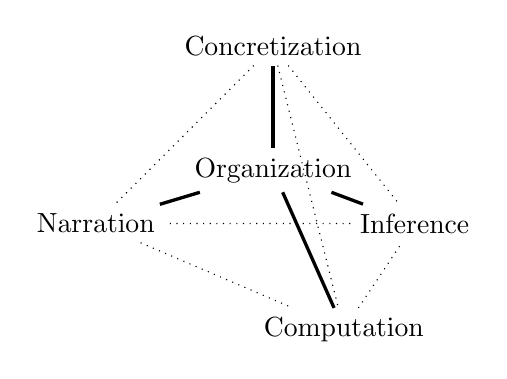
\begin{tikzpicture}[scale=\myscale]
  \node (center) at (0,.15) {Organization};
  \node (left) at (.2,-.3) {Computation};
  \node (right) at (.4,0) {Inference};
  \node (back) at (-.5,0) {Narration};
  \node (up) at (0,.5) {Concretization};

  \draw[very thick] (center) -- (left);
  \draw[very thick] (center) -- (right);
  \draw[very thick] (center) -- (back);
  \draw[very thick] (center) -- (up);
  \draw[dotted] (left) -- (right) -- (back) -- (left);
  \draw[dotted] (up) -- (left);
  \draw[dotted] (up) -- (right);
  \draw[dotted] (up) -- (back);
\end{tikzpicture}}
\caption{The tetrapodal structure of a mathematical software systems that supports the five aspects of doing mathematics. }
\label{fig:tetrapod}
\end{figure}

The organization aspect of mathematics is reflected in the efforts of building libraries of mathematics. The tetrapod project supports building a large library of mathematical knowledge organized as theory graph of biform theories~\cite{biformCICM2018}. The theory graph structure connects theories by describing how the symbols of a source theory can be interpreted in the target one. In a graph, one can express facts like `a group is a monoid` and that `monoid and additive monoid are isomorphic`. We explain theories, morphisms and graphs in more details in Chapter~\ref{ch:background}. 
Ideally, we want the nodes of the theory graph to be biform theories~\cite{biformCICM2018} which connect axiomatic theories  (used by theorem provers) and algorithmic theories (used by computer algebra systems) using meaning formulas. This way communication between reasoning and computation systems becomes possible. Communication can take the form reasoning about algorithmic theories or using results of computer algebra systems in theorem provers.\ednote{@WF: do biform theories still sound odd here?}  

This work contributes to the tetrapod project by investigating how a generative approach can contribute to building the library at the center of the tetrapod. We focus on building the algebraic hierarchy and the constructions related to the theories in it, mainly as described by universal algebra. The library we build has a theory graph structure, but the nodes are axiomatic, rather than biform, theories. 
%The theories we consider here are axiomatic theroies. that automatically generates a theory graph from theory expressions described in~\cite{carette2018building}. The nodes of this graph are axiomatic theories. We then work on the nodes of the graph to extract information from them. Finally, we make this information available in a agda. 
%There are different ways of organizing knowledge within a formal system. Our work contributes to building a large math library organized as a theory graph in the heart of a tetrapodal structure. Theory graphs, explained in details in Section~\ref{sec:background:theorygraph}, capture the structure of mathematical knowledge by enabling the description of relationships between the different pieces using morphisms. Using them, we can express facts like `a group is a monoid` and that `monoid and additive monoid are isomorphic`. 

%The nodes of a theory graph can be any kind of theories. Ideally, they would be biform theories~, as they connect axiomatic theories

%Morphisms are meaning preservation maps. The simplest form of a morphism is inclusion. Morphisms are used to transfer results from one theory to another. So, a morphism between \lstmath{Monoid} and \lstmath{AdditiveMonoid} that describes they are isomorphic, allows us to transfer results between them. 

%In, the authors argue that modern mathematics is organized as a tetrapod with knowledge organization being at its center. We are working towards a library organized as a theory graph of biform theories that serves as this center. Different aspects of the tetrapod will be consumers and producers of knowledge in this library. This implies that the size of this library would be huge, and that using generative approach to support its building would be a great asset. 

%We support the building of this library by providing combinators to define the library theories and algorithms to compute related constructions

\section{Publications}
This thesis lead to the following publications\ednote{Q: how should I refer to myself here, I? the author?}\ednote{Q: should I also include the abstract submitted to CICM2019 doctoral program?}: 
\begin{itemize}
    \item \cite{biformCICM2018} 
        \begin{itemize}
        \item[] contributed to writing the project description of biform theories, mainly the motivation. The project description appeared in the proceedings of CICM 2018. 
        \end{itemize}
    \item \cite{carette2018building} 
    \begin{itemize} 
    \item[] contibuted to an extended paper discussing the MathScheme combinators that were initially published in~\cite{CaretteOConnorTPC}. The extended paper is submitted to the journal of automated reasoning. I contributed to surveying related work and framing the novelty of the work with respect to them. I contributed to developing the type systems for the combinators. I also implemented the combinators as discussed here in Section~\ref{sec:lib_implementation}. I used my implementation to build a revised version of the MathScheme library. 
    %The development of the initial version of the library was part of the experiments~\cite{mathscheme2011experiments} that lead to the development of the combinators. To rebuild the library, we put some effort towards redefining the definitions that went wrong in the experiments. I also took part in developing the type systems for the combinators. 
%Surveying theory expressions in different formal systems to frame the novelty of the paper. 
%Taking part in developing the type system for the combinators 
%Providing the first arrow-based implementation of the paper, as we discuss in Section~\ref{sec:lib_implementation}. 
%Using the combinators to build a library of over $200$ theories. Although the library definitions pre-existed, many of them were not correct because they were based on theories. Shifting the implementation to arrows mandated figuring out the right arrows to build the theories, which was never done before this work.
   \end{itemize}
    \item ~\cite{diagrams_mmt} 
    \begin{itemize}
    \item[] used the diagram infrastructure developed in MMT~\cite{MMT} and described in the paper to implement the MathScheme combinators described in~\cite{carette2018building}. Since the combinators computes a theory and some arrows, we considered treating their inputs and outputs as diagrams.
This was an earlier attempt to implement the combinators and also the first time diagrams combinators in MMT are tested.  There were promising results, but did not scale up as - by that time - there were problems with how MMT supports the diagram combinators. 
    \end{itemize}        
    \item \cite{leverageCICM2020} 
    \begin{itemize}
    \item[]  presented redundancy in existing libraries and highlighted some of the problems we tackle in this thesis. Some of the main results of this thesis are published in the paper. I collected the examples of redundancy, implemented and tested the framework.
    \end{itemize} 
    \item \cite{bercic2020space} 
    \begin{itemize}
    \item[] contributed to surveying and categorizing how different mathematics software organize knowledge. Knowledge organization is one of $5$ categories of mathematics software the paper surveys. The other $4$ are inference, computation, concretization, and narration. 
%    The paper introduces a tetrapodal  organization of knowledge is in the cent paper discusses software used by producers and consumers of mathematical knowledge. 
    \end{itemize}        
\end{itemize}

\section{Outline}
We start by introducing some background knowledge in Chapter~\ref{ch:background}. We discuss the current practice of theory development within theorem provers, highlighting the redundancies that can be avoided in Chapter~\ref{ch:redundancy}. The methodology we use to remove those redundancies is introduced in Chapter~\ref{ch:design}. We present tog, the language and type checker that we use to develop our framework in Chapter~\ref{ch:tog}. The development of the algebraic hierarchy is presented in Chapter~\ref{ch:library}. In Chapter~\ref{ch:generation}, we discuss what information can be generated from theory presentations and how we extend tog to support generating them. We also present the constructions that we generate. The theories and the generated constructions are exported to Agda. We discuss the exporter in Chapter~\ref{ch:export}. 
We present related work in Chapter~\ref{ch:relatedwork}. Conclusion and future work are discussed in Chapter~\ref{ch:conclusion}. 
\todo{always check that this desciption of chapters still hold}

\begin{comment}  
These algebraic concepts are very important in mathematics and computer science that they are a main component in libraries of almost every mechanized system\ednote{add citations on research of algebra library development}. We consider the \lstmath{Monoid} structure for our running example. a \lstmath{Monoid} consists of a carrier over which there is an associative binary operation that has a unit. If we look at algebra textbooks, we find that~\cite{mckenzie1987algebras} defines it as 
\begin{quote}%[mathescape]
A monoid is an algebra $A = \langle \cdot^A, e^A \rangle$ such that 
$\langle A, \cdot^A \rangle$ is a semigroup and \\
$a \cdot^A e^A = e^A \cdot^A a = a$ for all $a \in A$.
\end{quote}
In~\cite{jacobson1985basic}, it is defined as 


Algebra text books would follow the definition of an algebraic structure with the definitions of some of its related constructions, like subalgebras, homomorphisms, term languages, quotients, etc. The scope of the book might determine which ones are included. \cite{jacobson1985basic} provides the following definition of monoid homomorphism 

and proceeds to talk about \lstmath{Group} homomorphism depending on the human ability to infer it from its given definition of \lstmath{Monoid}. 

Moving to formal systems, We find that they also do not agree on one definition of the theory \lstmath{Monoid}. Figure~\ref{fig:mon-diff-lang} shows its definition in $5$ different languages. 
\begin{figure}
\footnotesize
\begin{tabular}{p{6.3cm} p{7cm}}
\begin{lstlisting}[mathescape]
$\text{\underline{Haskell}}$
class Semiring a => Monoid a 
 where 
  mempty :: a 
  mappend :: a -> a -> a 
  mappend = (<>) 
  mconcat :: [a] -> a 
  mconcat = 
   foldr mappend mempty 
$\text{\underline{Coq}}$
class Monoid {A : type}
 (dot : A $\to$ A $\to$ A)
 (one : A) : Prop := {
  dot_assoc : forall x y z : A, 
  (dot x (dot y z)) = 
  dot (dot x y) z
  unit_left : forall x, 
  dot one x = x 
  unit_right : forall x, 
  dot x one = x              
}
$\text{\textit{Alternative Definition:}}$
Record monoid := {
 dom : Type; 
 op : dom -> dom -> dom 
  where "x * y" := op x y; 
 id : dom where "1" := id; 
 assoc : forall x y z, 
  x * (y * z) = (x * y) * z; 
 left_neutral : forall x,   
  1 * x = x; 
 right_neutal : forall x,
  x * 1 = x; 
}
$\text{\underline{MathScheme}}$
Monoid := Theory { 
 U : type; 
 * : (U,U) $\to$ U; 
 e : U; 
 axiom right_identity_*_e : 
  forall x : U $\cdot$ (x * e) = x;
 axiom left_identity_*_e :  
  forall x : U $\cdot$ (e * x) = x;
 axiom associativity_* : 
  forall x,y,z : U $\cdot$ 
  (x * y) * z = x * (y * z); 
}
\end{lstlisting}
&
\begin{lstlisting}[mathescape]
$\text{\underline{Agda}}$
record Monoid c $\ell$ : 
   Set (suc (c $\sqcup$ $\ell$)) where 
 infixl 7 _$\bullet$_
 infix 4 _$\approx$_
 field 
  Carrier : Set c 
  _$\approx$_ : Rel Carrier $\ell$ 
  _$\bullet$_ : Op$_2$ Carrier 
  isMonoid : IsMonoid _$\approx$_ _$\bullet$_ $\varepsilon$ 
$\text{where }$ IsMonoid $\text{ is defined as }$
record IsMonid ($\bullet$ : Op$_2$) ($\varepsilon$ : A) 
 : Set (a $\sqcup$ $\ell$) where 
  field 
   isSemiring : IsSemiring $\bullet$ 
   identity : Identity $\varepsilon$ 
       
   open IsSemigroup isSemigroup public 
   
   identity$^l$ : LeftIdentity $\varepsilon$ $\bullet$ 
   identity$^l$ = proj$_1$ identity 
   identity$^r$ : Rightdentity $\varepsilon$ $\bullet$ 
   identity$^r$ = proj$_2$ identity           

$\text{\underline{MMT}}$
theory Semigroup : ?NatDed = 
 u : sort 
 comp : tm u $\to$ tm u $\to$ tm u 
  # 1 * 2 prec 40
 assoc : $\vdash$ $\forall$ [x, y, z]
  (x * y) * z = x * (y * z)    
 assocLeftToRight : 
  {x,y,z} $\vdash$ (x * y) * z 
          = x * (y * z) 
  = [x,y,z] 
   allE (allE (allE assoc x) y) z
 assocRightToLeft : 
  {x,y,z} $\vdash$  x * (y * z) 
           = (x * y) * z 
  = [x,y,z] sym assocLR 
theory Monoid : ?NatDed 
 includes ?Semigroup 
 unit : tm u # e 
 unit_axiom : $\vdash$ $\forall$ [x] = x * e = x       
\end{lstlisting}       
\end{tabular}  

\caption{Representation of \lstinline|Monoid| theory in different languages.}
\label{fig:mon-diff-lang}
\end{figure}
For now, we imagine a definition of \lstmath{Monoid} in a simple language as follows 
\begin{lstlisting}[mathescape]
theory Monoid { 
A : type 
e : A
op : A $\to$ A $\to$ A
lunit : $\cdots$
runit : $\cdots$
assoc : $\cdots$ 
}
\end{lstlisting}        
The homomorphism of \lstmath{Monoid} in the same language is 
\begin{lstlisting}[mathescape]
theory MonoidHom { 
M1, M2 : Monoid  
hom : M1.A $\to$ M2.A 
pres-e : $\cdots$
pres-op : $\cdots$
}
\end{lstlisting}
The components of the homomorphism are $2$ instances of \lstmath{Monoid} theory, a mapping from the carrier of one instance to the other, and preservation axiom for every function symbols that follow the pattern 
\begin{lstlisting}[mathescape]
hom (op$_1$ x$_1$ .. x$_n$) = op$_2$ (hom x$_1$) .. (hom x$_n$)
\end{lstlisting}
Notice how all these components can be derived from the definition of \lstmath{Monoid}. 

Another commonly used algebraic structure is \lstmath{Group}. In order to use it in a formal system, one needs to define it along with all its related definitions that they need, like \lstmath{Group} homomorphism which follows the same pattern described above. This observation lead us to the question 
\end{comment}



\begin{comment}
Notice how all the 
~\cite{mckenzie1987algebras} is 
\begin{quote}%[mathescape]
A monoid is an algebra $A = \langle \cdot^A, e^A \rangle$ such that 
$\langle A, \cdot^A \rangle$ is a semigroup and \\
$a \cdot^A e^A = e^A \cdot^A a = a$ for all $a \in A$.
\end{quote}
Note how \lstmath{Monoid} is defined in terms of a smaller theory \lstmath{Semigroup}. While inthe definition given is  

In this case, \lstmath{Monoid} is defined in terms of its components. Both ways of defining \lstmath{Monoid} are useful and humans can switch between these definition without overhead. Depending on the task intended by the user, they might have a preference of one over the other. 
\end{comment}


%We focus our attention to algebra libraries which formalizes core concepts in mathematics and computer science. Algebra libraries contain axiomatic formalization of algebraic structures. Those structures describe classes of algebras. For example the algebras $(\mathbb{N},+,0)$ and $(Strings,++,\varepsilon)$ have similar behavior that is captured with the algebraic structure \lstmath{Monoid}. Defining and proofing properties of a structure is enough to define/prove it to all its models (all the algebras it describes). In the process of working with algebraic structures, one need some constructions related to them, like homomorphism, subalgebras, term algebras, etc. 


\chapter{Background}
\label{ch:background}
\todo{WF comment about equational FOL definition: the transitivity rule is not needed and the last rule is universal instantiation} 
\todo{conservative extensions: why would they act better under little theories than under big theories?}
In this chapter, we discuss some background concepts needed for presenting our work. 
Our ideas and implementation are based on dependent type theory (DTT). It is the meta theory for this work. We introduce it in Section~\ref{subsec:background:dtt} and define the notion of a theory and a context in Section~\ref{sec:background:theory}.
% Equational logic is based in set theory and forms the bases for universal algbera.  Dependent type theory (DTT) is a rich type theory in which types can depend on values. We want to represent theories of equational logic as contexts in DTT. We first introduce equational logic and DTT in Section~\ref{sec:background:logic}. 
%Contexts are defined in Section~\ref{sec:background:context} and theories in Section~\ref{sec:background:theory}. We then briefly introduce universal algebra and how it is used in our work in Section~\ref{sec:background:ualgebra}. 

Part of our work is building a library of axiomatic theories. The library is organized as a theory graph, in which theories are connected via morphisms. We introduce morphisms in Section~\ref{sec:background:morphisms} and discuss theory graphs and different strategies to building them in Section~\ref{sec:background:theorygraph}. 
To build the library we use combinators motivated by category theory, so we give a brief introduction for it in Section~\ref{sec:categoryTh}. 
One of the constructions we generate, that is not typically defined within universal algebra texts is multi-staged programming, so we define it in Section~\ref{sec:background:msp}. 

\section{Dependent Type Theory}
\label{subsec:background:dtt}
Dependent type theory (DTT) is a version of type theory that enables writing types like \lstmath{$\lambda\ $ x : A $\ \cdot\ $ M} where the type \lstmath{M} depends on the \emph{value} of \lstmath{x}. 
% source: Type theory and formal proof, P. 103 - Ch.5 
Having types that depends on values adds to the expressiveness of the logic. A common example for introducing dependent types is the type of a vector of \lstmath{n} elements of type \lstmath{A}. 
In most programming languages, the type of this vector is defined in terms of the type of its elements as \lstmath{Vec A}. Using dependent types, the type of a vector can depend on both the type of its elements and also its length, \lstmath{$\lambda\;$ n : Nat $\;\cdot\;$ Vec A n}, also written as \lstmath{$\Pi\;$ n : Nat $\;\cdot\;$ Vec A n}.
 
Having this extra piece of information in the type allow detection of some errors, like accessing out of bounds elements, on the type checker level. Type checking, then, guarantees that this kind of error does not exist in the given implementation. 
DTT has gained popularity and is used as 
Powerful type systems like DTT paves the way to building correct-by-construction software where the type of a function is its specification and type checkers are used to verify that the implementation follows the specification. 

%,  the specification is the type of the function 
%The descriptive power of DTT makes it more suitable for capturing mathematical knowledge. Therefore, many of the modern mechanized mathematics systems use variants of DTT as their foundations.\ednote{check this}  

\paragraph{$\Sigma$-types.}
A dependent pair, in which later elements depends on values of earlier ones, are referred to as $\Sigma$-types. The type \lstmath{$\Sigma\;$ (n : Nat, Vec A n)} refer to a pair that contains the value of \lstmath{n} in the first position and a vector of length \lstmath{n} in the second one. 

\paragraph{Telescopes.}
The concept of $\Sigma$ types is generalized into that of \emph{telescopes}, or equivalently,  \lstmath{dependent-type records}~\cite{pollack2002dependently}. A telescope $\mathbb{T}$ is defined as 
\begin{equation}
\mathbb{T} \equiv [x_1 : A_1][x_2 : A_2(x_1)][x_k : A_k(x_1,\cdots,x_{k-1})]
\label{eq:telescope}
\end{equation} 
The type \lstmath{Vec A n} as a telescope would be written as 
\lstmath{[A : Set][n : Nat][Vec A n]}. 
%Another related concept is the packaging of definitions in a structure in which a definition depends on earlier ones. This is called a dependent record type, and is referred to as $\Sigma$-types. The types \lstmath{A} and \lstmath{P:A $\;\to\;$ Type} can be grouped is a dependent pair $\Sigma A P$. 

%\section{Curry Howard Correspondence}
%Also known as propositions-as-types and proofs-as-programs, the Curry-Howard correspondence relates constructive logics, like dependent type theory, to computer programs.\ednote{expand this}.  

\paragraph{Contexts.}
%\label{sec:background:context}
In logic, A proposition is true if it is an axiom or is derivable from other true propositions using inference rules. This is usually written as $\varphi_1 ... \varphi_n \vdash \psi$.  In categorical logic, instead of talking about propositions, one talk about contexts. \cite{handbook1993CategoricalLogic} defines a context as 
\begin{quote}
A context, $\Gamma$, is a finite list $[x_1 : \sigma_1, ... , x_n : \sigma_n]$ of (variable,sort) pairs, subject to the condition that $x_1, ... , x_n$ is distinct.  
\end{quote}
When using dependent types, the context becomes a telescope, where every type in the list can contain reference to variables before it as described by Equation~\ref{eq:telescope}. The statement $\Gamma \vdash \psi$ means that the type judgement $\psi$ follows from the context $\Gamma$. The concatenation of two contexts $\Gamma_1$ and $\Gamma_2$ is noted by $\Gamma_1 ; \Gamma_2$.  
%\paragraph{The category of contexts}

\section{Theories}
\label{sec:background:theory}
%The set of formulas is called the language of the logic. The language is defined syntactically; there is no notion of meaning or semantics in a  logic per se. 
A theory  in some logic is defined as the tuple \lstmath{($\sort$,$\fsyms$,$\axioms$)} such that 
\begin{itemize}
\item $\sort$ is a set of sorts 
\item $\fsyms$ is a set of function symbols. 
\item $\axioms$ is the set of formulas that holds in $\Gamma$. 
\end{itemize}
The sort in $\sort$ and the function symbols in $\fsyms$ constitute the language of the theory. 
The set $\axioms$ is closed under logical consequence and usually infinite. 
A \emph{theory presentation} of some theory $\Gamma$ includes a finite set of sorts, a finite set of function symbols, and a finite set of generating axioms, i.e. axioms from which additional formulas can be derived by inference. 
Note that the same theory can have different theory presentations. 
In this work, as is traditionally the case, we use the term theory to refer to theory presentations. 
%Most algebra text books would refer to the language of the theory presentation as the signature and would separate its two components, writing it as \lstmath{(S,F)}. They often do not use the term \lstmath{theory}, but refer to sigantures with specific properties that are satisfied by the algebras. The use of axiomatic theories as we define them here is, to the best of our knowledge, tied to using them in computerized systems as in Clear~\cite{Goguen1980}. 

\paragraph{Theories as Contexts}
With dependent types and the Curry-Howard correspondance in place, the distinction between the three components of an axiomatic theory, sorts, function symbols, and axioms, is not needed anymore. Instead a theory is seen as a $\Sigma$ type, dependently-typed context, or a telescope as described by Equation~\ref{eq:telescope}. 
For example, the axiomatic formalization of \lstmath{Monoid} as a $\Sigma$ type is 
\begin{lstlisting}[mathescape]
$\Sigma$ (A : Set, $\Sigma$ (op : A $\;\to\;$ A $\;\to\;$ A, $\Sigma$ (e : A, 
  $\Sigma$ (lunit : {x : A} $\;\to\;$ op e x = x,
    $\Sigma$ (runit : {x : A} $\;\to\;$ op x e = x,
      $\Sigma$ (assoc : {x y z : A} $\;\to\;$ op x (op y z) = 
                                op (op x y) z))))))
\end{lstlisting} 
which can be describe as a telescope as  
\begin{togcode} 
Monoid = [A : Set, op : A ~$\;\to\;$~ A ~$\;\to\;$~ A, e : A, 
          lunit : {x : A} ~$\;\to\;$~ op e x = x, 
          runit : {x : A} ~$\;\to\;$~ op x e = x, 
          assoc : {x y z : A} ~$\;\to\;$~ op x (op y z) = op (op x y) z] 
\end{togcode} 
This definition induces a context from which the type \lstmath{op e e = e} can be defined, which is noted as \lstmath{Monoid $\ \vdash\ $ triv : op e e = e}  

%The telescopic representation of a sort would be \lstmath{$\sort$:$\square$} where $\square$ is a kind defined in the type theory. A function symbol within a telescope is defined in terms of the type of its parameters. Propositions-as-types make it possible to present axioms as part of telescopes. is declared as $\sort : Type$. 
%Every declaration \lstmath{c:t} within the telescope is defined within a context \lstmath{$\Gamma$}. This is described as \lstmath{$\Gamma \vdash\;$ c:t}. 

%Theories in DTT are seen as contexts. This is how they are presented in~\cite{carette2018building} which forms the basis of this work. Therefore, we use the term context to also mean a theory in DTT. 

A theory presentation is well-typed if every declaration \lstmath{c:t} is well-typed given its context. The formation rules for theory presentations are given in Figure~\ref{fig:ctx}, where $\syms{\Gamma}$ refers to the list of symbols defined in the context $\Gamma$. 
$$ \syms{\context{\varnothing}} = \EmptyThy \qquad
\syms{\context{\Gamma}\ ;\ x : \sigma} = \syms{\context{\Gamma}} \cup \left\{ x \right\}
$$
\begin{figure}[ht]
    \begin{proofrules}
        \[ \ \justifies \varnothing \ \wfctx \]
        \[ \context{\Gamma}\ \wfctx \qquad \sigma \notin \syms{\context{\Gamma}}
        \qquad \context{\Gamma} \vdash \kappa : \Box \justifies
        (\context{\Gamma}\ ;\ \sigma : \kappa)\ \wfctx \]
        \[ \context{\Gamma}\ \wfctx \qquad x\notin \syms{\context{\Gamma}}
        \qquad \context{\Gamma} \vdash \sigma : \kappa : \Box \justifies
        (\context{\Gamma}\ ;\ x : \sigma)\ \wfctx \]
    \end{proofrules}
    \caption{Formation rules for contexts as introduced in~\cite{carette2018building}}
    \label{fig:ctx}
\end{figure}

\section{Theory Morphisms}
\label{sec:background:morphisms}
Morphisms are used to capture the structure of mathematics, by describing how theories are related to each other. In mathematical texts, a theorem proved for an arbitrary \lstmath{Monoid} can be used when considering an arbitrary \lstmath{Group} without extra work. Formally, this can be done if a meaning preserving morphism between \lstmath{Monoid} and \lstmath{Group} exists. The morphism specifies how results in \lstmath{Monoid} can be interpreted in \lstmath{Group}. 

A morphism $\arrow{[v]}{\Gamma}{\Delta}$ consist of a list of assignments $[v]$, a source theory \lstmath{$\Gamma$}, and a target theory \lstmath{$\Delta$}. $[v]$ assigns to every symbol in $\Gamma$ an expression of $\Delta$. A term \lstmath{t} in the language of $\Gamma$ can be translated into a term \lstmath{t$^\prime$} in the language of $\Delta$ using substitution, such that  \lstmath{t$^\prime$ = t$[v]$}. Using the morphism 
\lstmath{[op to + ; e to 0] : Monoid $\;\to\;$ AdditiveMonoid}
we are able to interpret the expression \lstmath{(op e x)} in \lstmath{Monoid} as \lstmath{(+ 0 x)} in \lstmath{AdditiveMonoid} using substitution. 
%For example, a morphism from \lstmath{Monoid} to \lstmath{AdditiveMonoid} contains the assignments \lstmath{op to +} and \lstmath{e to 0} 

The formation rules for views, as given in~\cite{carette2018building} is given in Figure~\ref{fig:views}. 
\begin{figure}[ht]
    \begin{proofrules}
        \[ \context{\Delta}\ \wfctx \justifies \view{}{\varnothing}{\Delta} \]
        \[ (\context{\Gamma}\ ;\ x : \sigma)\ \wfctx \qquad
        \view{v}{\Gamma}{\Delta} \qquad
        \context{\Delta} \vdash r : \substitution{\sigma}{v}{} \justifies
        \view{v,x \mapsto r}{(\context{\Gamma}\ ;\ x : \sigma)}{\context{\Delta}} \]
    \end{proofrules}
    \caption{Formation rules for morphisms.}
    \label{fig:views}
\end{figure}

It is worth mentioning that the mapping is only a part of the morphism. A morphism consists of the source and destination theories as well as the mapping, i.e. the same substitution can induce different morphisms as the source and target are modified. 

Connecting theories have been known for a long time in logic~\cite{tarski1953undecidable, enderton1972mathematical} under the name \emph{theory interpretations}. The same name is used by IMPS~\cite{farmer1993imps, InterpIMPS1994}. Clear~\cite{Goguen1980}, OBJ and their successors used the term \emph{morphisms}, maybe because of using category theory for semantics. The term \emph{view} has also been used to refer to the same concept by Maude, MathScheme, and MMT. In this work, we use the terms views and morphisms interchangeably. 

We distinguish between three type of morphisms 

\subsection{Identity Morphism}
\label{sec:idmorph}
If $\arrow{[v]}{\Gamma}{\Delta}$ is an identity morphism, then $[v]$ maps every symbol $x \in \syms{\Gamma}$ to itself such that $x[v] = x$.
%This implies that $[v]$ is a bijection and that . 
While it is common to name source and target of identities with the same name, we do not do that here as $\Gamma$ and $\Delta$ are two different theory presentations. The identity between them means that symbols in $\Gamma$ are interpreted the same way in $\Delta$. 

Identity morphisms exist between two theories if the source is included verbatim in the destination, like in the case when \lstmath{Group} is defined as an extension of \lstmath{Monoid}. It is the simplest form of morphisms and allow transport of results without the need to perform substitution 

\subsection{Embedding}
\label{sec:embedding}
If $\arrow{[v]}{\Gamma}{\Delta}$ is an embedding, then $[v]$ maps every symbol $x \in \syms{\Gamma}$ to a symbol $r \in \syms{\Delta}$, which is not necessarily itself. 

Consider for example, the following morphism from \verb|Magma| to \verb|AdditiveMagma|
\begin{equation*}\label{eq:additiveview}
\begin{tikzpicture}[node distance=9.0cm, auto,baseline=(current bounding box.center)]
\node (P) {$
    \begin{thyex}
    \thyrow{A}{\tmop{Type}}
    \thyrow{op}{A \rightarrow A \rightarrow A}
%    \thyrow{assoc_op}{\cdots}
    \end{thyex} $};
\node (B) [right of=P] {$
    \begin{thyex}
    \thyrow{A}{\tmop{Type}}
    \thyrow{+}{A \rightarrow A \rightarrow A}
%    \thyrow{assoc_+}{\cdots}
    \end{thyex} $};
\draw[->] (P) to node {$[A \mapsto\ A, 
    op \mapsto\ + ]$} (B);
\end{tikzpicture}
\end{equation*}
A term $t \in \Gamma$ is transported to $\Delta$ as $t[v]$, i.e.: by applying the substitution $[v]$ to the term $t$. 
So if \lstmath{$t =\;$ op x y}, then using the morphism above it is transported to $\Delta$ as \lstmath{(+ x y)}. 

We refer to an embedding morphism as $\tilde{m}$, and therefore identity morphisms are referred to as $\tilde{id}$. 

\subsection{General Morphism}
\label{sec:generalmorph}
A morphism $\arrow{[v]}{\Gamma}{\Delta}$ is a general morphism if it maps symbols $x \in \syms{\Gamma}$ to terms $r \in \Delta$. 

An example is a morphism that flips a binary operation, i.e.: maps \lstmath{op x y} to \lstmath{op y x}
\begin{equation}\label{eq:flipmagmaview}
\begin{tikzpicture}[node distance=9.0cm, auto,baseline=(current bounding box.center)]
\node (P) {$
    \begin{thyex}
    \thyrow{A}{\tmop{Type}}
    \thyrow{op}{A \rightarrow A \rightarrow A}
    \end{thyex} $};
\node (B) [right of=P] {$
    \begin{thyex}
    \thyrow{A}{\tmop{Type}}
    \thyrow{op}{A \rightarrow A \rightarrow A}
    \end{thyex} $};
\draw[->] (P) to node {$[A \mapsto\ A,
    op \mapsto\ \mathsf{flip}\ op]$} (B);
\end{tikzpicture}
\end{equation}

%\section{Substitution}
%Morphisms acts on theories by substitution, i.e.: Given a morphism $[v] : \Gamma \to \Delta$, by performing the substitution of mappings in $[v]$ to symbols in $\Gamma$, we get the presentation $\Delta$. This substitution is written as $\Gamma[v]$. 
%Mappings acts on theories by substitution, i.e.: Given a list of assignments of terms to symbols $[x \mapsto y]$ and an expression e, a substitution replaces every free occurence of $x$ in the theory by y. 

\section{Theory Graph}\label{sec:background:theorygraph}
One way to organize theories is using theory graphs. A theory graph is a directed acyclic graph consisting of theories as nodes and morphisms as edges between them. It is helpful in managing large libraries~\cite{kohlhase2010towards}.

In systems that are based on categorical semantics, a theory graph is seen as a diagram in the category of theories and theory morphisms. Specware~\cite{Smith99} uses the keyword \emph{diagram} to build them. The work in~\cite{developmentGraph2000}, based on CASL, refer to them as \emph{development graphs}. 

Organizing a library as a theory graph leverages the structure of mathematics by relying on morphisms to connect the different concepts presented within the theories. Compare a library defining the graph leading to  \lstmath{Monoid} as in Figure~\ref{fig:cube_monoid} to one that defines it only in terms of its components, as in Section~\ref{sec:background:theory}. The theory graph one has more information which makes it more useful to library users. 
Theory graphs also makes it possible to modularize a formalization by adding definitions or proving theorems within smaller modules (theories). Definitions and theorems are then made available to different other theories by transporting them via morphisms. 

Here we discuss two strategies for decomposing theories; little and tiny theories.  

%By comparing the theory graph in Figure~\ref{fig:cube_monoid} with a definition of \lstmath{Monoid} in terms of its declarations shows how using a graph to define \lstmath{Monoid} leverages i
  
%Theory graphs leverage the structure of mathematics by relying on morphisms to connect the different concepts presented within the theories. 
%This way it is possible to add definitions and proof theorems within one theory 
%Therefore, it becomes possible to decompose definitions and proofs to pieces of knowledge into smaller contexts and perform reasoning within these contexts. In cases when this knowledge is needed in a different context, then transport them to different ones when needed. we are able to decompose the development of theories. Having morphisms also facilitates the transportation of results between theories. 

\subsection{Little Theories}
The little theories approach is introduced in~\cite{LittleTheories}. The idea is to ensure that if a statement \lstmath{s} is proven in context \lstmath{$\Gamma$}, then every statement in \lstmath{$\Gamma$} is required to prove \lstmath{s}. In this case, we say \lstmath{$\Gamma$} is the \emph{minimal axiomatization} needed to prove \lstmath{s}. This implies that theorems are proved in different contexts based on the amount of structure needed to prove them. In contrast, the big theory approach would a small set of big theories for proving all results\footnote{Or a medium-sized set of medium-sized theories}. 

Using little theories increases the reuse of results. For example, if the theorem \lstmath{op e e = e} is proven in the theory \lstmath{Unital}, it can be transported to all theories that are connected to \lstmath{Unital} via morphisms, like \lstmath{Monoid}. On the other hand, if it is proven in the theory \lstmath{Group}, it cannot be transported to \lstmath{Monoid}, because all declarations in \lstmath{Group} becomes part of the context for proving the theorem.  
%to a less number of theories under the assumption that \lstmath{Group} is defined from \lstmath{Unital} using a series of extensions. 
%Results proven in the theory \lstmath{$\Gamma$} can be transported to all theories \lstmath{$\Delta$} whenever a morphism $m : \Gamma \to \Delta$ exists. 
% increasing usability and reducing redundancy when dealing with formal systems.  

\subsection{Tiny Theories}
\label{sec:background:tinytheories}
Tiny theories is a refinement of little theories, in which only one new piece of information is added at a time~\cite{mathscheme2011experiments}. To make this more clear, let's consider a library that has the theories \lstmath{PointedMagma} and \lstmath{Unital} defined as follows. \\
\begin{tabular}{p{7cm} p{7cm}}
\begin{lstlisting}[mathescape, basicstyle=\footnotesize]
theory PointedMagma = { 
  A : Type 
  e : A 
  op : A $\to$ A $\to$ A }
\end{lstlisting}
&
\begin{lstlisting}[mathescape, basicstyle=\footnotesize]
theory Unital = {
  A : Type 
  e : A 
  op : A $\to$ A $\to$ A 
  lunit : {x : A} $\to$ op e x = x
  runit : {x : A} $\to$ op x e = x   }   
\end{lstlisting}
\end{tabular}
Defining \lstmath{Unital} this way overlooks that in some cases one might want to define a theory to describe structures with a carrier and a binary operation on it that has only a right unit, like a theory with Integers as carrier and subtraction as the only binary operation. 
One will then need to add a new theory that is similar to \lstmath{Unital} without the \lstmath{lunit} declaration. Any theorems proved in the context of \lstmath{Unital} cannot be used, even if it only depends on \lstmath{runit}. 

Using tiny theories, one would first define a \lstmath{LeftUnital} theory adding the \lstmath{lunit} axiom to \lstmath{PointedMagma}, a \lstmath{RightUnital} theory adding \lstmath{runit} axiom, and the theory of \lstmath{Unital} would be connected to both \lstmath{LeftUnital} and \lstmath{RightUnital}, creating more connections and therefore, allowing more reuse of results. Systematically using tiny theories to develop a large library leads to the need for support to diamond structures, which we discuss in Chapter~\ref{ch:library} based on the work in \cite{carette2018building}.  

\section[Category Theory]{Category Theory\footnote{This section is based on~\cite{pierce1990taste}}}
\label{sec:categoryTh}
Category theory is a foundational framework, like set and type theory, that is abstract and structured enough to allow hidden commonalities of concepts to emerge. 

While set theory has elements of sets as the main concept, category theory is built around the concept of morphisms. The source and target of a morphism are objects in the category. Category theory is not concerned with the internal structure of the objects, but rather by how they relate to other objects. 

A category $\mathcal{C}$ consists of 
\begin{itemize}
\item A collection of objects, $\syms{\mathcal{C}}$
\item A collection of morphisms between the objects. A morphism is represented as $u : \Gamma \to \Delta$.  
\item Operations assigning to every morphism to its domain and codomain 
\item A composition function $\cdot$ assigning to each pair of morphisms  $u : \Gamma \to \Delta$ and $v : \Delta \to \Phi$, a morphism $u \cdot v : \Gamma \to \Phi$, such that 
\[ u \cdot (v \cdot w) = (u \cdot v) \cdot w \]
\item For every object $\Gamma$ in $\mathcal{C}$, an identity morphism $id_\Gamma : \Gamma \to \Gamma$, such that for $u : \Gamma \to \Delta$ 
\[ id_\Gamma \cdot u = u \cdot id_\Delta = u \]
\end{itemize}

Finite categories can be represented diagrammatically as in Figure~\ref{fig:diagram}. 
\begin{figure}
\centering{
\begin{tikzcd}
 & \Gamma \arrow[loop] \arrow[dr]& \\
\Delta \arrow[loop left] \arrow[rr] \arrow[ur] & & \Phi \arrow[loop right] 
\end{tikzcd}}
\caption{A diagram in a category with at least $3$ objects}
\label{fig:diagram}
\end{figure}
Such a diagram is said to commute if for every pair of vertices, $\Gamma$ and $\Delta$, all paths from $\Gamma$ to $\Delta$ are equal. 

In the following we introduce two concepts related to categories that we use in Chapter~\ref{ch:library}. These are pushouts and colimits. \cite{nlab:colimit} gives an intuition of what a colimit is as 
\begin{quote}
``The intuitive general idea of a colimit is that it defines an object obtained by sewing together the objects of the diagram, according to the instructions given by the morphisms of the diagram"
\end{quote}
A pushout is a special case of a colimit. In~\cite{nlab:pushout}, it is mentioned that 
\begin{quote}
``A pushout is the colimit of the diagram 
\begin{tikzcd} 
\bullet & \bullet \arrow[l] \arrow[r] & \bullet
\end{tikzcd}"
\end{quote}
The formal definitions of the two constructions are
\paragraph{Pushouts.}
The pushout of a pair of arrows $u_\Delta : \Gamma \to \Delta$ and $u_\Phi : \Gamma \to \Phi$ is an object $\Xi$ and a pair of arrows $v_\Delta : \Delta \to \Xi$ and $v_\Phi : \Phi \to \Xi$ such that 
\begin{itemize}
\item $u_\Delta \cdot v_\Delta = u_\Phi \cdot v_\Phi $
\item for morphisms $w_\Delta : \Delta \to \Omega$ and $w_\Phi : \Phi \to \Omega$, there is a unique $w : \Xi \to \Omega$, such that 
$v_\Delta \cdot w = w_\Delta$ and $v_\Phi \cdot w = w_\Phi$
\end{itemize}
The definition of the pushout is illustrated in Figure\ref{fig:pushoutDef}. 
\begin{figure}
\centering{
\begin{tikzcd} 
\Gamma \arrow["u_\Delta",d] \arrow["u_\Phi",rr]& & \Phi \arrow["v_\Phi",d] \arrow["w_\Phi",rdd, bend left] \\
\Delta \arrow["v_\Delta",rr] \arrow["w_\Delta",rrrd, bend right]& & \Xi \arrow[dashed, rd] \\ 
& & & \Omega
\end{tikzcd}} 
\caption{Diagram illustrating the definition of a pushout}
\label{fig:pushoutDef}
\end{figure}

\paragraph{Colimits.}
Colimits are defined in terms of cocones. The definitions we present here are adapted from~\cite{sannella2012foundations}. 

A cocone over a diagram consists of an object $\Gamma$ and a family of morphisms $u_0 : \Delta_0 \to \Gamma, ..., u_n : \Delta_n \to \Gamma$, where $n$ is the number of nodes in the diagram other than $\Gamma$, such that for every morphism $v : \Delta_i \to \Delta_j$ in the diagram $v \cdot u_j = u_i$, i.e. the following diagram commutes 
\begin{tikzcd} 
& \Gamma & \\ 
\Delta_i \arrow[ur,"u_i"] \arrow[rr,"v"] & & \Delta_j \arrow[ul,"u_j"] 
\end{tikzcd}
The notation used to descrine cocones is 
$\langle u_i : \Gamma \to \Delta_i \rangle_{i\leq n}$.

The colimit of a diagram is a cocone  
$\langle u_i : \Gamma \to \Delta_i \rangle_{i\leq n}$ such that for any cocone 
$\langle u_i^{\prime} : \Gamma^{\prime} \to \Delta_i \rangle_{i\leq n}$ there is a unique morphism $v : \Gamma \to \Gamma^\prime$ such that for every $u_i$, the following diagram commutes 
\begin{tikzcd} 
\Gamma \arrow[ rr,dashed, "v"] && \Gamma^\prime \\ 
& \Delta_i \arrow[ul,"u_i"] \arrow [ur," u_i^{\prime}"] & 
\end{tikzcd} 

\section{Multi-Staged Programming}
\label{sec:background:msp}
Meta-programming is the practice of writing \emph{meta} programs that manipulate \emph{object} programs. Meta and object programs can be in the same or different languages. Generative programming is one form of meta-programming in which the meta-program compiles into a program of the object language. Therefore, the process of running the meta-program involves two stages, compile and run-time. 

The meta program might need to refer to code in the object language, like in the case of making a call to a predefined function in the object language. In this case, the meta program is deferring the evaluation of this code to a \lstmath{later} stage. 
Also, a meta program might need to evaluate a meta or object language expression that results in an object code. In this case, the expression is evaluated in the \lstmath{current} stage. 

In our implementation, we define two stages \lstmath{s0} and \lstmath{s1}. 
\begin{togcode}
data Stage : Set where
  s0 : Stage
  s1 : Stage
\end{togcode} 

Staging an expression means adding annotation to its components indicating which stage it should be evaluated in. 
\lstmath{Now} or \lstmath{Later}. 
\begin{togcode} 
data Staged (A : Set) : Set where
  Now : A -> Staged A
  Later : Comp A s1 -> Staged A
\end{togcode} 
Annotating an expression of type \lstmath{A} with the \lstmath{Now} constructor indicates that it will be evaluated in the current stage and a value of type \lstmath{A} is promised to exist. On the other hand, if the evaluation is deferred to \lstmath{Later}, then the expression will have the type \lstmath{Comp}, for computation. 
\begin{togcode} 
data Comp (A : Set) (s : Stage) : Set where
  Computation : Choice -> CodeRep A s -> Comp A s
\end{togcode} 
Computations encapsulate quoted fragments of code. The \lstmath{CodeRep} function assigns a stage \lstmath{s0} or \lstmath{s1} to the expression. 
\begin{togcode} 
data Wrap (A : Set) : Set where
  Q : A -> Wrap A
CodeRep : (A : Set) (s : Stage) -> Set
  CodeRep A s0 = A
  CodeRep A s1 = Wrap (CodeRep A s0)
\end{togcode} 
We also add a flag indicating whether the quoted code represent an expression (\lstmath{Expr}) or a literal, constant or variable (\lstmath{Const}).  
\begin{togcode} 
data Choice : Set where
  Expr : Choice
  Const : Choice
\end{togcode} 

There are $3$ main applications to staging; generating well-typed code as in MetaOcaml~\cite{taha1999multi}, removing abstraction overhead introduced by generic programming~\cite{yallop2016StagingGeneric, carette2011mspFunctorsMonads, carette2011generative}, and developing domain specific languages~\cite{sheard2000stagingDSL}. MetaOcaml and Haskell templates provide staging constructs under the names \emph{quote} and \emph{eval} instead of \emph{Now} and \emph{Later}. In logical reasoning the same ideas are used for reflection, as in~\cite{farmer2013quoteEval}.  


%MSP gives the developers of the meta program the control over it by annotating which pieces can be evaluated at runtime\ednote{better writing}.  
%Writing program generators typically involve multiple stages; generation, compilation, and runtime stage. 
%MSP is a technique for managing code generation across different stages until execution. to provide annotations for the generator 

%\section{Finally Tagless}
%\label{sec:background:tagless}
%While staging is useful in so many ways, it introduces the overhead of dealing with the tags to \lstmath{Now} and \lstmath{Later}, or \lstmath{quote} and \lstmath{eval}. The finally tagless approach aim to remove this tagging overhead by encoding the object language as functions within a class, instead of constructors of a datatype. For example, the language of monoid would be represented as a type by: 


\chapter{Universal Algebra}
\label{ch:ualgebra}
Algebraic structures, like monoids, groups, and rings studies classes of algebra that have similar properties. Universal algbera studies algebras in a more generic way. It abstracts over the specific properties of classes of algebras and deals with them as axiomatic theories in equational first-order logic. With this abstraction in place, universal algebra define some constructions useful when dealing with algebras and prove some of their properties.

We use concepts of universal algebra to leverage the information in theory presentations. We internalize a representation of uni-sorted equational first order theories into DTT, our meta theory. This way we are able to manipulate them and generate the constructions as described by universal algebra. In this chapter we introduce core concepts that we use from universal algebra. In Chapter~\ref{ch:generation} we discuss how we use it in our work. In Section~\ref{sec:eqtheory} we present equational first order logic, the meta theory for universal algebra, and define the components of a theory in this logic. We then introduce some of the constructions of universal algebra that can be generated from an equational theory presentation in Section~\ref{sec:toBeGenerated}. It is worth mentioning that although our framework generate only some of these constructions, they all follow from the definition of a theory and the definitions we provide here will hopefully make this noticeable.   

\section{Equational Theory}
\label{sec:eqtheory}
Logics give us the machinery to describe properties of entities as formulas and reason about them.  
Equational logic restricts these formulas, whether axioms or theorems, to be equations of the form \lstmath{t$_1$ = t$_2$}, where \lstmath{t$_1$} and  \lstmath{t$_2$} are terms expressible in the language of the theory. There are different notions of equality~\cite{oneThingSame2008, equalityInTPs2015}. In many cases the underlying logic offers its own equality. In some other cases, the equality is defined by the language of the theory, as is the case with setoids. 

Equational logic has $3$ inference rules described in~\cite{Gries1993EquationalLogic}\ednote{@WF: waiting for your recommendation on a better reference for equational FOL}  
\begin{proofrules}
        \[ t_1 = t_2 \ \justifies t[x \mapsto t_1] = t[x \mapsto t_2] \]
        \[ t_1 = t_2 , t_2 = t_3 \ \justifies t_1 = t_3 \]
        \[t \ \justifies t [xs \mapsto ts] \] 
\end{proofrules}       
where $t$, $t_1$, $t_2$, and $t_3$ are expressions, $x$ is a symbol in the language, $ts$ is a list of expressions, and $xs$ is a list of symbols. 
The leftmost rule refers to leibniz equality that states that two expressions are equal if one can be substituted by the other without changing the truth of a statement. 
The rule in the middle reflects the transitivity of equality. 
The rightmost rule states that if $t$ is true under all assignments, then it is true under any valid substitution.  

%\section{A Theory in Equational Logic} 
%\label{sec:eqtheory}
A theory in universal algebra is described in first order equational logic. It restricts the definition of a theory described in Section~\ref{sec:background:theory}. It is defined as a tuple \lstmath{($\sort$,$\fsyms$,$\equations$)}
such that 
\begin{itemize}
\item $\sort$ is a set of one sort \lstmath{s}. 
\item $\fsyms$ is a finite set of function symbols. 
\item $\equations$ is a finite set of generating equations. 
\end{itemize}
%containing one sort .\footnote{In case of multi-sorted logics, the set $\sort$ is an indexed set of sorts. We restrict ourselves to unisorted logics as it captures the algebraic structures we're interested in, like monoids, groups, and rings.}
%An equation has the form \lstmath{t$_1$ = t$_2$}. We refer to this set as $\equations$, and therefore refer to a theory in equational logic as \lstmath{($\sort$,$\fsyms$,$\equations$)}. 


\section{Constructions}
\label{sec:toBeGenerated}
%Algebra makes the basis of many areas of computer science. We are interested in theorem proving and specification systems. \ednote{relate this to the background section} \ednote{uniform notation and citation} In many places the term algebra is used to refer to the 
The definition of an equational theory captures various algebraic structures. To effectively use these structures, universal algebra provide us with definitions of constructions related to them.  we will describe some of these constructions here. We use the $\sort$ symbol to refer to the one sort in the set. The definitions are adapted from~\cite{ehrig1985fundamentals} and~\cite{handbook1993Maibaum}.  

\begin{itemize}
    \item The \emph{signature} of a theory $(\sort, \fsyms, \equations)$ is $(\sort, \fsyms)$ consisting of the sort and $n$-ary function symbols, where $n \geq 0$. The signature specifies the language of the theory, without any laws. 
    \item The \emph{product} of two algebras \lstmath{A} and \lstmath{B} of the same theory $\Gamma$ is the algebra with sort $(\sort_A \times \sort_B)$. In a uni-sorted setup, the sort of the product algebra is $(\sort \times \sort)$. 
    \begin{itemize}
    \item \lstmath{c$_\times$ : $(\sort \times \sort)$}, for every constant symbol 
      \lstmath{c $\;\in\;\mid\Gamma\mid$}. 
    \item \lstmath{op$_\times$ : $(\sort \times \sort) \to \cdots \to (\sort \times \sort)$}, for every function symbol \lstmath{op $\;\in\; \mid\Gamma\mid$} based on its arity. 
    \item The set of equations $\equations_\times$ is given by substituting the new sort, constant and function symbols in the set $\sort$.  
    \end{itemize}
    \item The \emph{sub-theory} $\Delta$ of a theory $\Gamma$ is defined as 
    \begin{enumerate}
    \item $\sort_\Delta \subseteq \sort_\Gamma$ 
    \item \lstmath{c$_\Delta$} \lstmath{=} \lstmath{c$_{\Gamma}$} for every constant symbol in the set of function symbols $\fsyms$. 
    \item \lstmath{op$_\Delta\ $ x$_1$ $\;...\;$ x$_n$} \lstmath{=} \lstmath{op$_\Gamma\ $x$_1$ $\;...\;$ x$_n$}, for all \lstmath{op$\ \in\;\mid\fsyms\mid$}, {x$_1$ $\cdots$ x$_n$ $\in \sort$}, and \lstmath{n $\ \in \mathbb{N}$, n $\;\geq\;$ 1}. 
    \end{enumerate}
    \item The \emph{trivial sub-theory} is the subtheory with the empty carrier. Because the carrier is empty, the $3$ axioms above trivially hold. 
    \item The \emph{homomorphism} between two algebras \lstmath{A} and \lstmath{B} of the same theory $\Gamma$ is a function \lstmath{hom : $\;\sort_A \to \sort_B$} such that 
    \begin{itemize}
        \item for every constant symbol in $\fsyms$: \lstmath{hom c$_A$ = c$_B$} 
        \item for every function symbol in $\fsyms$: 
           \lstmath{hom (op$_A\ $ x$_1$ $\;\cdots\;$ x$_n$) = op$_B\ $ (hom x$_1$)  $\;...\;$ (hom x$_n$)} 
    \end{itemize}
    There are some variants of homomorphism that can be easily generated from it. These variants are  
    \begin{itemize}
    	\item \emph{monomorphisms} are injective homomorphisms 
  	  	\item \emph{epimorphisms} are surjective homomorphisms 
    	\item \emph{endomorphisms} are homomorphisms from an object to itself 
    	\item \emph{isomorphisms} are bijective homomorphisms. 
    	\item \emph{automorphisms} are isomorphisms from an object to itself. 
    \end{itemize}
    \item The \emph{kernel} of a homomorphism from algebra \lstmath{A} to algebra \lstmath{B} of the same theory $\Gamma$ is defined as the binary relation \lstmath{$\equiv_{hom}$} on the sort of \lstmath{A}, such that 
    \begin{lstlisting}[mathescape] 
    a $\equiv_{hom}$ b $\Leftrightarrow$ hom a $\equiv_{hom}$ hom b
    \end{lstlisting}
    for every \lstmath{a} and \lstmath{b} in $\sort_A$. 
    \item The composition of two morphisms \lstmath{f : A $\ \to\ $ B} and \lstmath{g : B $\ \to\ $ C} is denoted by the function \lstmath{g $\ \circ\ $ f : A $\ \to\ $ C} and is defined as 
    \lstmath{(g $\ \circ\ $ f) a = g (f a)} for every \lstmath{a $\ \in\ $ A}   
 %   \item Homomorphism Equality 
    \item The \emph{relational interpretation} between two algebras \lstmath{A} and \lstmath{B} of the same theory is a relation \lstmath{interp a b}, for all \lstmath{a $\;\in \sort_A$} and \lstmath{b $\;\in \sort_B$} such that 
    \begin{itemize}
    \item interp c$_A$ c$_B$, for every constant \lstmath{c $\;\in\;$ A}.  
    \item interp x$_1$ y$_1$ $\ \wedge\ $ $\ \cdots\ $ $\ \wedge\ $ interp x$_n$ y$_n$ $\Rightarrow$ interp (op$_A$ x$_1$ $\ \cdots\ $ x$_n$) (op$_B$ y$_1$ $\ \cdots\ $ y$_n$) for all function symbols \lstmath{op $\;\in \mid\fsyms\mid$}, where \lstmath{x$_1$ $\; ... \;$ x$_n$ $\ \in\ $ $\sort_A$} and \lstmath{y$_1$ $\; ... \;$ y$_n$ $\;\in \sort_B$}. 
    \end{itemize}
    
    \item The \emph{quotient algebra} for a theory $\Gamma$ with respect to some congruence relation \lstmath{$\equiv$} is defined as the theory \lstmath{$\Gamma/\equiv \;= (\sort_Q, \fsyms_Q, \equations_Q)$} such that\ednote{Q: How to define \lstmath{E$_{Q}$}} 
    \begin{itemize}
       \item \lstmath{$\sort_Q$} is the factor set of $\sort$, defined as 
       	\begin{lstlisting}[mathescape]
       	$\sort_Q$ = {[x] $\mid$ x $\in \sort$}
       	\end{lstlisting} 
       	where \lstmath{[x]} is the equivalence class defined as \lstmath{[x] = $\{$y $\ \in \sort \mid\ $ x $\ \equiv\ $ y$\}$}
       \item \lstmath{c$_Q$ = [c]}, for constant symbols \lstmath{c $\ \in\fsyms$} and \lstmath{c$_Q$ $\ \in \fsyms_Q$}.  
       \item \lstmath{f$_Q$ [x$_1$] $\ \cdots\ $ [x$_n$]} = [f x$_1$ $\ \cdots\ $ x$_n$]
       for function symbols \lstmath{f$_Q$ $\ \in \fsyms_Q$} and \lstmath{f $\ \in \fsyms$}.
    \end{itemize}      

%    \item congruence of functions 
%    \item The monotonicity of a function 
    \item The \emph{closed term language} induced by a theory is a set of terms that are defined inductively as 
    \begin{itemize}
        \item all constants belong to the language (basic terms) 
        \item A term \lstmath{t$_{\texttt{op}}$ $\ $ t$_1$ $\ \cdots\ $ t$_n$} for every function symbol \lstmath{op : $\sort \to ... \to \sort $} of arity $n$, such that  \lstmath{t$_1$ $\ \cdots\ $ t$_n$} belongs to the language. 
    \end{itemize}
    \item The \emph{open term language} of a theory is similar to the closed term language, except that basic terms includes a set of variables.  
    \item The \emph{staged term language} of a theory is the term language in which expressions can be marked for execution in compile or runtime stages as discussed in Section~\ref{sec:background:msp}.  
    \item Structural induction: Let \lstmath{p} be a predicate defined on terms \lstmath{t $\ \in\ $ T$_{\texttt{op}}$(X)} of a signature \lstmath{SIG = $(\sort,\fsyms)$} with a set of variables \lstmath{X}. The assertion \lstmath{p(t)} is true for all \lstmath{t $\ \in\ $ T$_{\texttt{op}}$} if the following conditions are satisfied: 
    \begin{itemize}
        \item \lstmath{p(t)} is true for all constant and variable symbols 
        \item for each term \lstmath{f t$_1$ $\ \cdots\ $ t$_n$}, we have that if \lstmath{(p t$_1$) $...$ (p t$_n$)} are true, then also \lstmath{p (f t$_1$ $\ \cdots\ $ t$_n$)} is true.  
    \end{itemize}     
    \item Evaluation functions: Given an algebra \lstmath{A} of a theory \lstmath{$\Gamma = (\sort,\fsyms,\equations$)}, a term of the language of the theory as defined above, the function \lstmath{eval : T$\;\to \sort_\texttt{A}$} is defined recursively as 
    \begin{itemize}
        \item \lstmath{eval c = c$_{A}$}
        \item \lstmath{eval (op t$_1$ $\ \cdots\ $ t$_n$)} = op$_A$ (eval t$_1$) $\cdots$ (eval t$_n$) where an assignment function maps the constants of the language to the constants defined by the algebra. The evaluation function for open term language would be similar except it has an additional environment that assigns value of the carrier to variables. 
    \end{itemize}      
    \item Simplification via rewriting: Given a set of equations, each represented as \lstmath{(X,L,R)}, where \lstmath{X} is a set of variables, \lstmath{L} is the term on the left of the equation, and \lstmath{R} is the term on the right side. By fixing the set of variables, we can represent equations as  (L,R). Each equation represented this form gives rise to two substitutions \lstmath{1) L $\ \Rightarrow\ $ R} and \lstmath{2) R $\ \Rightarrow\ $ L}. Any of these substitutions can result in rewriting systems, but when simplifying one need to define an ordering relation that decides which term is \emph{simpler} than the other. When having the equations and the ordering relation, rewriting systems can be defined. 
    \item Equivalence of terms: two terms can be denoted equal in one or more of the following cases 
    \begin{itemize}
        \item by calling the eval function on both terms they yield the same value.  
        \item by calling the simplify function on both terms they yield the same value. 
        \item using structural equivalence, the two terms have the same parse tree. 
    \end{itemize}
    \item A printing function similar to the show function in haskell. 
  %  \item Applying functors to terms: 
    \item Setters and getters for instances of data types (lenses in Haskell). the same way haskell does it to data types using template haskell. 
%    \item Theory Actions 
 %   \item Subset Actions
 %   \item Coset of a theory 
\end{itemize}
We give the definitions of these constructs based on set theory, as one would find them in a standard text book. It has been formalized in type theory in  both Coq in~\cite{capretta99, Spitters2010} and agda~\cite{Gunther2018Agda}. In~\cite{capretta99}, the formalization of algebraic structures in type theory is done using record types. 
%A reddit post have observed that these structures can be generated~\cite{redditGenHom}. The discussion went on\ednote{continue this} and~\cite{agdaGenPull}

% -------------------------------------------------------------- 
%\section{Logic}
%\label{sec:eqlogic}
\begin{comment} 
A logic, as in ~\cite{Gries1993FormalLogic}, is a set of rules defined in terms of 
\begin{itemize}
\item a set of symbols, like \lstmath{=}, \lstmath{$\wedge$}, \lstmath{$\vee$}, constants, like \lstmath{true} and \lstmath{false}, and variables, like \lstmath{p} and \lstmath{q}. 
\item a set of formulas constructed from the symbols.  
\item a set of axioms stating the properties of the symbols  
\item a set of inference rules used to derive new formulas.  
\end{itemize}
The language of the logic provides the meta-symbols that theories in that logic uses to formulate their languages and formulas. Logics give the tools to model entities of the world by writing formulas to describe them. These formulas are either axioms or theorems that are proven by applying inference rules to the axioms. A sound set of rules would guarantee that only true statements are derived. 
Logics have different expressive powers. In this work we are interested in equational logic and dependent type theory.
\end{comment}  

\chapter{Theory Development Practice}
\label{ch:redundancy}

The formal systems community has mostly focused on making necessary things possible. Our focus is more oriented to making uniform definitions free. In this chapter we highlight the redundancy that is currently a part of the development of theories in formal systems. In Section~\ref{sec:redun:libraries} we focus our attention to libraries of formal systems, while in Section~\ref{sec:redun:user_projects} we show how some projects are redfines algebraic structure and some other constructions because they are unable to use the definitions provided by libraries of the system they are using. 

\section{Algebra Theories in Libraries}\ednote{currently a copy-paste from the paper}
\label{sec:redun:libraries}

One of our observations is that current formalizations of Algebra contain quite a
bit of information that is ``free'' in the sense that it can be
mechanically generated from basic definitions. For example, given a theory
X, it is mechanical to define X-homomorphisms. To do this within a system
is extremely difficult, as it would require introspection and for theory
\emph{definitions} to be first-class citizens, which is not the case for any
system based on type-theory that we are aware of. Untyped systems
in the Lisp tradition do this routinely, as does Maude~\cite{Maude}, which
is based on \emph{rewriting logic}; the downside is that there is no
difference between meaningful and meaningless transformations in these
systems, only between ``runs successfully'' and ``crashes''. However,
these constructions are fully typeable and, moreover, are not system-specific
(as they can be phrased meta-theoretically within Universal
Algebra), even though an implementation has to be aware of the syntactic
details of each system.

Lest the reader think that our quest is a little quixotic, we first look at
current libraries from a variety of systems, to find concrete examples of
human-written code that could have been generated. We look at Agda,
Isabelle/HOL and Lean in particular. More specifically, we look at
\href{https://github.com/agda/agda-stdlib/releases/tag/v1.3}
{version 1.3 of the Agda standard library},
the \href
{https://isabelle.in.tum.de/website-Isabelle2019/dist/library/HOL/HOL-Algebra/index.html} 
{2019 release of the Isabelle/HOL library}
and 
\href
{https://github.com/leanprover-community/mathlib/releases/tag/snapshot-2019-10}
{Lean's mathlib}, where we link to the proper release tag.

We use the theory \verb|Monoid| as our running example, and we 
highlight the reusable components that the systems use to make writing the
definitions easier and more robust. 

\subsection{Homomorphism}
How do the libraries of our three systems\footnote{We do not have enough room
    to give an introduction to each system; hopefully each system's syntax is
    clear enough for the main ideas to come through.}
represent homomorphism?

\subsubsection{Agda}
defines \lstmath{Monoid} homomorphism, indirectly, in two ways. First,
a predicate encapsulating the proof obligations is defined, which is
layered on top of the predicate for 
\href
{https://github.com/agda/agda-stdlib/blob/4a8d8f5ffbdbd967ca1bb708895ea63709e0063d/src/Algebra/Morphism.agda} 
{Semigroup homomorphism}.
This is then used to define homomorphisms themselves.

\begin{agdacode}
module _ {c~$_1$~ ~$\ell_1$~ c~$_2$~ ~$\ell_2$~}
(From : Monoid c~$_1$~ ~$\ell_1$~)
(To   : Monoid c~$_2$~ ~$\ell_2$~) where

private
module F = Monoid From
module T = Monoid To

record IsSemigroupMorphism (~$\llbracket$~_~$\rrbracket$~:Morphism)
: Set(c~$_1$~ ~$\sqcup$~ ~$\ell_1$~ ~$\sqcup$~ c~$_2$~ ~$\sqcup$~ ~$\ell_2$~) where 
field
~$\llbracket\rrbracket$~-cong : ~$\llbracket$~_~$\rrbracket$~ Preserves F._~$\approx$~_ ~$\to$~ T._~$\approx$~_
~$\bigdot$~-homo  : Homomorphic~$_2$~ ~$\llbracket$~_~$\rrbracket$~ F._~$\bigdot$~_ T._~$\bigdot$~_
~$\cdots$~
record IsMonoidMorphism (~$\llbracket$~_~$\rrbracket$~:Morphism)
: Set(c~$_1$~ ~$\sqcup$~ ~$\ell_1$~ ~$\sqcup$~ c~$_2$~ ~$\sqcup$~ ~$\ell_2$~) where 
field
sm-homo : IsSemigroupMorphism F.semigroup T.semigroup ~$\llbracket$~_~$\rrbracket$~
~$\varepsilon$~-homo   : Homomorphic~$_0$~ ~$\llbracket$~_~$\rrbracket$~ F.~$\varepsilon$~ T.~$\varepsilon$~

open IsSemigroupMorphism sm-homo public
\end{agdacode}

There are many design decisions embedded in the above definitions. These
decisions are not canonical, so we need to understand them to later
be able to both abstract them out and make them variation points in our
generator. Namely, these decisions are:
\begin{itemize}
    \item The choice of which declarations are parameters and which are fields.
    The monoids (\verb|From| and \verb|To|) over which we define homomorphism
    are parameters, not fields, as is the function
    \lstinline[mathescape]|$\llbracket$_$\rrbracket$|.
    \item The preservation axioms can be defined based on their arity
    patterns, as type-level function such as
    \lstinline[mathescape]|Homomorphic$_{2}$|:
    \begin{agdacode}
Homomorphic~$_{2}$~ : (A ~$\to$~ B) ~$\to$~ Op~$_2$~ A ~$\to$~ Op~$_2$~ B ~$\to$~ Set _ 
Homomorphic~$_{2}$~ ~$\llbracket$~_~$\rrbracket$~ _~$\bigdot$~_ _~$\circ$~_ =
  ~$\forall$~ x y ~$\to$~ ~$\sembr{\text{ x } \bigdot \text{ y }}$~ ~$\approx$~ (~$\sembr{\text{ x }}$~ ~$\circ$~ ~$\sembr{\text{ y }}$~)
    \end{agdacode}
    The library also provides shortcuts for $0$-ary and $1$-ary function
    symbols, the most common cases.
    \item The definition of structures over setoids. Thus equalities need 
    to be preserved, and that is what the 
    \lstinline[mathescape]|$\llbracket\rrbracket$-cong| axiom states.
\end{itemize}

\subsubsection{Isabelle/HOL}
provides the following definition of \href{https://isabelle.in.tum.de/website-Isabelle2019/dist/library/HOL/HOL-Algebra/Group.html}{monoid homomorphism}:

\begin{isabellecode}
definition  _ ~$\Rightarrow$~ _ ~$\Rightarrow$~ ('a ~$\Rightarrow$~ 'b) set where 
hom G H =
  {h ~$\cdot$~ h ~$\in$~ carrier G ~$\to$~ carrier H ~$\wedge$~ 
  (~$\forall$~ x ~$\in$~ carrier G ~$\cdot$~ ~$\forall$~ y ~$\in$~ carrier G  ~$\cdot$~ 
    h (x ~$\oplus_\text{G}$~ y) = h x ~$\oplus_\text{H}$~ h y)}
\end{isabellecode}
\ednote{The problem of minted accpeting double quotes}

The reader might notice a discrepancy in the above: unit preservation is
missing.  The Isabelle library does not provide this version.
There is, however, a proof that such a multiplication-preserving homomorphism
necessarily maps the source unit to a unit of the image (sub)monoid, but that
unit is not necessarily that of the full image. The above definition is also
used to define group homomorphism and other structures. We consider
this to be missing information in the library. 


\subsubsection{Lean}\hspace{-0.4em}'s
definition of \href{https://github.com/leanprover-community/mathlib/blob/3c58f160fd51ebf989138ed7c8981f821f08f860/src/algebra/group/hom.lean}
{monoid homomorphism}
is the one that most resembles the one found in textbooks. 
\begin{leancode}
structure monoid_hom (M : Type*) (N : Type*) 
[monoid M] [monoid N] :=
(to_fun : M ~$\to$~ N)
(map_one' : to_fun 1 = 1)
(map_mul' : ~$\forall$~ x y, to_fun (x * y) = to_fun x * to_fun y)
\end{leancode}

However, in the same file, there is another definition of \verb|add_monoid_hom| that looks ``the same'' up to renaming. This points
to a weakness of Lean: there is no renaming operation on 
\verb|structure|, and for a \verb|Ring| to contain two ``monoids'', one
is forced to duplicate definitions. This redundancy is unpleasant.

\subsection{Term Language}

The ``term language'' of a theory is the (inductive) data type
that represents the syntax of well-formed terms of that theory,
along with an interpretation function from \emph{expressions} 
to the carrier of the (implicitly single-sorted) given theory, i.e.
its denotational semantics.

In Agda, the definition of \lstinline|Monoid| term language is straightforward:
\begin{agdacode}
data Expr (n : ~$\mathbb{N}$~) where 
var : Fin n ~$\to$~ Expr n 
id : Expr n 
_~$\oplus$~_ : Expr n ~$\to$~ Expr n ~$\to$~ Expr n 
\end{agdacode}
Defining the interpretation function requires the concept of an environment.
An environment associates a value to every variable, and the semantics
associates a value (of type \verb|Carrier|) to each expression of \verb|Expr|.
\begin{agdacode}
Env : Set _ 
Env = ~$\lambda$~ n ~$\rightarrow$~ Vec Carrier n 

~$\llbracket$~_~$\rrbracket$~ : ~$\forall$~ {n} ~$\to$~ Expr n ~$\to$~ Env n ~$\to$~ Carrier 
~$\llbracket$~ var x ~$\rrbracket$~ ~$\upvarrho$~ = lookup ~$\upvarrho$~ x 
~$\llbracket$~ id ~$\rrbracket$~ ~$\upvarrho$~ = ~$\epsilon$~ 
~$\llbracket$~ e~$_1$~ ~$\oplus$~ e~$_2$~ ~$\rrbracket$~ ~$\upvarrho$~ = ~$\llbracket$~ e~$_1$~ ~$\rrbracket$~ ~$\upvarrho$~ ~$\cdot$~ ~$\llbracket$~ e~$_2$~ ~$\rrbracket$~ ~$\upvarrho$~ 
\end{agdacode}


In Agda, these definitions are not found with the definitions of the
algebraic structures themselves, but rather as part of the
\emph{Solver} for equations over that theory. Here, we find more
duplication, as the above definitions
are repeated for the following three highly related structures: 
\href{https://github.com/agda/agda-stdlib/blob/4a8d8f5ffbdbd967ca1bb708895ea63709e0063d/src/Algebra/Solver/Monoid.agda}
{\lstinline|Monoid|},
\href{https://github.com/agda/agda-stdlib/blob/4a8d8f5ffbdbd967ca1bb708895ea63709e0063d/src/Algebra/Solver/CommutativeMonoid.agda}
{\lstinline|CommutativeMonoid|}
and 
\href{https://github.com/agda/agda-stdlib/blob/4a8d8f5ffbdbd967ca1bb708895ea63709e0063d/src/Algebra/Solver/IdempotentCommutativeMonoid.agda}
{\lstinline|IdempotentCommutativeMonoid|}.

Despite its usefulness, we were not able to find the definition of the term
language of a theory in Isabelle/HOL or Lean.  

\subsection{Product}
Until recently, there was no definition of the product of algebraic
structures in the Agda library.  A 
\href{https://github.com/agda/agda-stdlib/pull/1109}{recent pull request}
has suggested adding these, along with other constructions.  The
following hand-written definition has now been added:
\begin{agdacode}
rawMonoid : RawMonoid c c~$\ell$~ ~$\to$~ RawMonoid d d~$\ell$~ ~$\to$~ 
RawMonoid (c ~$\sqcup$~ d) (c~$\ell$~ ~$\sqcup$~ d~$\ell$~)
rawMonoid M N = record
{ Carrier = M.Carrier ~$\times$~ N.Carrier
; _~$\approx$~_ = Pointwise M._~$\approx$~_ N._~$\approx$~_
; _~$\bigdot$~_ = zip M._~$\bigdot$~_ N._~$\bigdot$~_
; ~$\varepsilon$~ = M.~$\varepsilon$~ , N.~$\varepsilon$~
}
where
module M = RawMonoid M
module N = RawMonoid N
\end{agdacode}

These could have been mechanically generated from the definition
of \verb|Monoid|.

Both 
\href{https://isabelle.in.tum.de/website-Isabelle2019/dist/library/HOL/HOL-Algebra/Group.html}
{Isabelle/HOL}
and 
\href{https://github.com/leanprover-community/mathlib/blob/3c58f160fd51ebf989138ed7c8981f821f08f860/src/algebra/pi_instances.lean}
{Lean}
provide definitions of product algebras for monoids, which we omit for space.
It is worth mentioning that the Lean library has $15$ definitions for products
of structures that look very similar and could be generated. 


\section{Algebra Theories in User Projects}
\label{sec:redun:user_projects}

We continue investigating the redundancy in code written by developers. In the previous section we looked into general purpose libraries. We now turn our attention to user projects highlighting the cases when users had to redefine information already existing in libraries. 

The theories and data structures project~\cite{theoriesAndDts}, implemented in Agda, explores how algebraic theories give rise to some common data structures. A natural first step is to formalize the algebraic theories of interest to the project. Despite the existence of some of these algebraic structures in the standard library, like the \lstmath{Monoid} theory with the definition above, the project developers redefined many of them~\footnote{https://github.com/JacquesCarette/TheoriesAndDataStructures/tree/master/Structures}, like \lstmath{Magma, }\lstmath{Monoid}, \lstmath{CommMonoid}, and \lstmath{AbelianGroup}. In some cases, like in \lstmath{Monoid}, the definitions avoided setoids, while in others, like in \lstmath{CommMonoid} it used it. This highlights how important it is to provide a way of customizing definitions while using them. 

The MGG project~\cite{carette2011generative} deals with the computational geometry software as a family of programs and aim to define abstractions from which different software pieces can be generated. One of the layers common to many members of this software family is algebra. In \lstmath{Algebra.lhs} the finally tagless representation of many algebraic structures are given as follows 
\begin{hscode}
class Monoid repr n where
  add :: repr n -> repr n -> repr n
  zero :: repr n

class Monoid repr n => AdditiveGroup repr n where
  neg :: repr n -> repr n
  sub :: repr n -> repr n -> repr n
  int_pow :: Integer -> repr n -> repr n
  of_int :: Integer -> repr n
\end{hscode}
We show in Chapter~\ref{ch:generation} that the finally tagless representation can be generated. Another form of redundancy, is defining the \lstmath{Monoid} instance of various number representations, like float, integer and rational, along with the code and staged versions. For example, in Float.lhs, we find the following definition 
\begin{hscode}
instance Monoid BaseImm Double where
  add = liftA2 (+)
  zero = pure (0.0)

instance Monoid Code Double where
  add (Code x) (Code y) = Code [| $(x) + $(y) |]
  zero = Code [| 0.0 |]

instance Monoid Staged Double where
  add a b = monoid Alg.zero add add a b
  zero = of_atom (0.0)
\end{hscode}
with instances of the three version of \lstmath{Double} for \lstmath{Field}, \lstmath{AdditiveGroup}, \lstmath{Norm}, and \lstmath{Ring}. The same definitions in repeated for \lstmath{Integer} type in Integer.lhs file. 
\begin{hscode}
instance Monoid BaseImm Integer where
  add = liftA2 (+)
  zero = pure 0

instance Monoid Code Integer where
  add (Code x) (Code y) = Code [| $(x) + $(y) |]
  zero = Code [| 0 |]

instance Monoid Staged Integer where
  zero = of_atom $ 0
  add = monoid A.zero add add
\end{hscode}
and for rationals in Rational.lhs\ednote{Problem with this example is the repo has limited accessibility.}




\chapter{Tog: Language and Type Checker}
\label{ch:tog}

%The interpreter of our DSL generates definitions of theories and related constructions. 
To implement the methodology we presented in Chapter~\ref{ch:design}, we need a language for representing and manipulating theories and a type checker to verify these manipulations. 
Theories are written in some formal language, the object language. To manipulate them we need to investigate and manipulate the syntax of the object language. This can be done in the same language if it has a strong reflection mechanism, or in the meta language in which the object language is embedded. As the main goal of our work is to investigate the usefulness of a generative approach, we do not want to be constrained by the amount of support given by the reflection mechanism. Working in the meta language gives us full control over manipulating the object language's syntax. 
We need our meta language to support the following features in the object language it represents:
\begin{itemize}
\item $\Pi$-Types: The semantics of the combinators we are using is given in categorical dependent logic. Having $\Pi$-types is needed to represent the types of views in terms of their source and target theories. 
\item Dependent records to represent theories as telescopes. 
\item A module system to manage namespaces such that every theory with its generated constructions is a module. 
\item Inductive data types to represent term languages. 
\item Equality to represent the equations within a theory. 
\end{itemize}

These features are available in most dependently typed systems, like Agda, Coq, and Lean. But we refrained from using any of these systems to avoid delving into their design decisions. Instead, we prefer a small language that does not have many other extra features. We use Tog~\cite{tog}, a small implementation of Martin-L\"{o}f type theory. 
It provides a small dependently typed language and type checker. It was created by the Agda developers to experiment with type checking ideas. It has mainly been used to experiment with type checking through unification~\cite{mazzoli2016type}. 

Tog is implemented in Haskell. Figure~\ref{fig:togRepr} shows its internal representation. 
% , style=trac
\begin{figure}
\begin{minted}[fontsize=\scriptsize,escapeinside=~~,mathescape=true]{haskell}
data Decl
    = TypeSig TypeSig
    | FunDef Name [Pattern] FunDefBody
    | Data Name Params DataBody
    | Record Name Params RecordBody
    | Module_ Module
    | ~$\cdots$~
    deriving (Eq, Ord, Show, Read)

data TypeSig = Sig Name Expr
    deriving (Eq, Ord, Show, Read)

data Where = Where [Decl] | NoWhere
    deriving (Eq, Ord, Show, Read)

data Params
    = NoParams | ParamDecl [Binding] | ParamDef [HiddenName]
    deriving (Eq, Ord, Show, Read)

data HiddenName = NotHidden Name | Hidden Name
    deriving (Eq, Ord, Show, Read)

data DataBody
    = DataDecl Name | DataDef [Constr] | DataDeclDef Name [Constr]
    deriving (Eq, Ord, Show, Read)

data RecordBody
    = RecordDecl Name
    | RecordDef Name Fields
    | RecordDeclDef Name Name Fields
    deriving (Eq, Ord, Show, Read)

data Fields = NoFields | Fields [Constr]
    deriving (Eq, Ord, Show, Read)

data Constr = Constr Name Expr
    deriving (Eq, Ord, Show, Read)

data FunDefBody = FunDefNoBody | FunDefBody Expr Where
    deriving (Eq, Ord, Show, Read)

data Telescope = Tel [Binding]
    deriving (Eq, Ord, Show, Read)

data Binding = Bind [Arg] Expr | HBind [Arg] Expr
    deriving (Eq, Ord, Show, Read)

data Expr
    = Lam [Name] Expr
    | Pi Telescope Expr    -- $\Pi$ types 
    | Fun Expr Expr        -- function types  
    | Eq Expr Expr         -- equations 
    | App [Arg]            -- type applications 
    | Id QName             -- types names
    deriving (Eq, Ord, Show, Read)

data Arg = HArg Expr | Arg Expr
    deriving (Eq, Ord, Show, Read)

data Pattern
    = EmptyP Empty | ConP QName [Pattern] | IdP QName | HideP Pattern
    deriving (Eq, Ord, Show, Read)
\end{minted}
\caption{Internal Representation of the Tog Language}
\label{fig:togRepr}
\end{figure}

A Tog module is a list of declarations, such that each declaration is either a type signature, function definition, datatype declaration, record definition, or a nested module represented using the  \lstmath{TypeSig}, \lstmath{FunDef}, \lstmath{Data}, \lstmath{Record}, and \lstmath{Module$\_$} constructors, respectively. 
According to the type \lstmath{Decl}, modules can import and open other modules, but our experience shows that this feature is not supported. 

Parameters to modules, records, and datatypes are represented by the \lstmath{Params} type. A single parameter has type \lstmath{Binding} and can be declared implicit by using the constructor \lstmath{HBind}. 

A record field and a datatype constructor are both of type \lstmath{Constr}, each having a name and a type expression \lstmath{Expr}. Dependent types are created with the \lstmath{Pi} constructor. Function types are curried and represented with the \lstmath{Fun} constructor. Axioms that are equations are represented with \lstmath{Eq} constructor. Type and function applications are created using the \lstmath{App} constructor. If a type has no arguments, then the \lstmath{Id} constructor is used to refer to it by name. 

To perform pattern matching, the \lstmath{Pattern} type is used. Matching with a $0$-ary constructor is done using \lstmath{IdP}. If the constructor takes parameters, then \lstmath{ConP} is used. \lstmath{HideP} represents pattern matching on implicit arguments and \lstmath{EmptyP} represents the don't care \lstmath{$\_$} character. 

We extend Tog to support the input theory expressions and flatten them into Tog dependent records and morphisms between them. 
The structure of these dependent records is used to generate new constructions. The generated constructions can be records, datatypes, or functions presented in Tog syntax. The well-typedness of the generated constructions is ensured by the Tog type checker. 

%The fact that tog has no universes (Set : Set). that we couldn't find a better experimental language, and that this would not affect the generated constructions because we do not perform any reasoning and our code is backed by universal algebra, so we have a meta theory that tell us that we are not generating nonsense 
%\ednote{We probably need to say something about universes in Tog. In tog, it is true that \lstmath{Set : Set}. We decided then that this is not a big deal, but I don't know why.}



\chapter{Framework Design}

Building DSLs is useful in achieving many software qualities. In case of library building, some of the benefits include:  
\begin{itemize}
    \item More readable definitions for mathematicians 
    \item Better customizable definitions for user of mechanized systems 
    \item Less labor from the side of library developers 
    \item Better maintainability of library 
\end{itemize}

The interpreter of a DSL transforms declarative expressions into definitions acceptable by a host language. We suggest an interpreter that consists of three phases as shown in Figure~\ref{fig:staged-interpreter}. 
\begin{figure}
\includegraphics[scale=0.5,width=\linewidth]{figures/interpreter_detailed}
\caption{A $3$-staged interpreter for generating libraries}
\label{fig:staged-interpreter}
\end{figure}

\paragraph{Flattener.} The first stage of the interpreter take in theory expressions and computes a flat version of the theory being described. The theory expressions need to be designed well enough to describe the structure of mathematics, i.e. build a theory graph paying special attention to morphisms that describes how theories relate to each other. Describing this structure is useful in transporting results, but mathematical results are not always shaped in terms of the hierarchy. A \lstmath{Group} can be described as a \lstmath{Monoid} with inverse or as a structure with binary and unary operatoins that have some properties. Our library need to support both definitions, by enabling the users to work with flat version of the library. Some operations on theories make this hard to achieve, like dropping and freeness combinators by CASL\ednote{look for a source explaining why they are problematic}. 
\ednote{add a figure?}

\paragraph{Generator.} When we have a flat theory presentation describing an algebraic structure, we check if this theory falls under the abstraction provided by universal algebra. The algebraic hierarchy until at least \lstmath{Ring}\ednote{or maybe more?} does. If so, then we are able to generate the constructions that universal algebra describes based on that abstraction. 

\paragraph{Exporter.} Variabilities in the design decisions between different systems affects how theory presentations look like. At the end of the day, those variabilities are translated into syntactic differences. By abstracting over them, we are able to remove or add them upon the developer's will. It is the job of the exporter to do that, providing a version of the theory that fits best the users' purposes. 





\chapter{A Library of Algebraic Structures}
\label{ch:library}
%One can define a new theory either by stating its components or by using combinators to build it from existing ones. 

In this Chapter, we build a library of axiomatic theories representing the algebraic hierarchy. 
%before we use it to generate related constructions that we discuss in Chapter~\ref{ch:generation}. 
Our library consists of equational first-order theories organized as a theory graph using the tiny theories approach. Instead of having to provide all declaration of the theories and morphisms within the graph, we use the MathScheme combinators introduced in~\cite{CaretteOConnorTPC, carette2018building}. 

It is common to see the algebraic hierarchy as a series of inclusions as in Figure~\ref{fig:flatExtensions}. 
\begin{figure}
\centering{
\begin{tikzcd}
\cn{Magma} \arrow[r, hook] & \cn{Semigroup}\arrow[r, hook] & \cn{Monoid} \arrow[r, hook] & \cn{Group} \arrow[r, hook] & \cdots
\end{tikzcd}}
\caption{Algebraic structures as extensions.}
\label{fig:flatExtensions}
\end{figure}  
But the algebraic hierarchy is richer than that, considering for example the list in~\cite{jipsen}. 
In Section~\ref{sec:background:tinytheories} we discuss tiny theories as an adequate approach to building a theory graph that captures this structure. The nodes of the graph are theory presentations and they are connected via morphisms (see Section~\ref{sec:background:theorygraph}). Morphisms describe how the different theory presentations relate to each other. 
We present the example of building the theory of \lstmath{Unital} by extending the theory of \lstmath{PointedMagma} to create \lstmath{LeftUnital} and \lstmath{RightUnital}, then combining them. This example is described by a diamond structure as in Figure~\ref{fig:unitalDiamond}. 
\begin{figure}
\centering{
\begin{tikzcd} 
& \verb|LeftUnital| \arrow[dr,hook] & \\
\verb|PointedMagma| \arrow[ur,hook] \arrow [dr,hook] & & \verb|Unital| \\
& \verb|RightUnital| \arrow[ur,hook] &
\end{tikzcd}}
\caption{The diamond in the definition of \lstmath{Unital}.}
\label{fig:unitalDiamond}
\end{figure}
The diamond structure appearing in the definition of \lstmath{Unital} is not a special case. Instead, diamonds are pervasive in the algebraic hierarchy, as shown in the theory graph for defining \lstmath{Monoid} in Figure~\ref{fig:cube_monoid}. 
%examining the work in \cite{halleck} and \citeauthors{jipsen} show us that the algebraic %hierarchy is more packed with diamonds, as we show in Figure~
%As we discussed in Section~\ref{sec:thry_graph_in_action}, dealing with diamonds is a challenging problem~\cite{sakkinen1989disciplined, jigsaw1992, traits2006, diamonds2011}. There is a gap in how specification systems handle them, whether by not following its correct semantics, or by not supporting it at all. 

But the diamond structure does not come without problems. We need to have careful infrastructure to deal with them in order to avoid the diamond problem~\cite{jigsaw1992,traits2006,diamonds2011}, a.k.a. multiple inheritance or the fork-join problem~\cite{sakkinen1989disciplined}, which we discuss in Section~\ref{subsec:combine}.

In Section~\ref{sec:thry_graph_in_action} we provide an overview of the support for morphisms in different formal systems. Section~\ref{sec:msCombinators} introduces the MathScheme combinators for a morphism-based approach to building theory graphs, leading to a solution to the diamond problem. We discuss how to use the combinators to build the library in Section~\ref{sec:guidelines}. We end up with Section~\ref{sec:library:discussion} discussing best practice for using the combinators. 

\begin{comment}
To test our generation algorithms, we needed a large library of equational theories. As we have discussed in Section~\ref{sec:broader_context}, we work in the favor of a library organized as a theory graph, believing that it leverages the structure of mathematical knowledge. Morphisms of the graph are the means to relating the different theories. In this section, we present our approach to building a library that emphasizes these connections. 

In Section~\ref{sec:thry_based_libs} we discuss the motivation behind building such a library. In Section~\ref{sec:ms_combinators} we present the combinators used in building it and discuss how they are morphism based. Section~\ref{sec:lib_implementation}, discusses the challenges of the implementation of the combinators to build a theory graph. We finally show some interesting cases of library definitions in Section~\ref{sec:interesting_cases}. 
\end{comment}


\section{Theory Graph Development}
\label{sec:thry_graph_in_action}

Although many formal systems support theory graph structures, more support for using and defining morphisms is needed. 
Specware~\cite{Smith99} and MMT~\cite{MMT} force users to provide all details of theories and morphisms between them. IMPS~\cite{farmer1993imps}, in some cases, generates morphisms given source and target theories. 

%On the other hand, it leads to a multiple diamonds (a.k.a. multiple inheritance) in the development of the hierarchy. 
%Many formal systems support a theory graph approach, and realizes the need of having morphisms between theories. Examples of these are Clear, OBJ, CASL, Maude, Specware, IMPS, and MMT. 

%Clear is - to our knowledge - the first system that provides a modular way to write formal specifications. It provide theory combinators to build larger theories from smaller ones. 
%\ednote{A good resource for Clear is the PhD thesis of Sanella with the title: semantics, implementation and pragmatics of CLEAR} 
Another way to support building a library rich in morphisms is to provide combinators to handle some of the work. Clear~\cite{Goguen1980} is --- to our knowledge --- the first system to use combinators for creating new theories\footnote{Clear is a specification language, and theories are used under the name specifications.}. OBJ~\cite{Obj2000Goguen} and CASL~\cite{CoFI:2004:CASL-RM} are successors of Clear that also support combinators. We focus our discussion on CASL as a representative to these systems, as it is the only living one now and so we were only able to look at its library and run experiments on it. 
We realized two problems related to combinators in CASL. First, it is not always possible to flatten theories built through the use of combinators, especially hiding and freeness combinators~\cite{CoFI:2004:CASL-RM}. The second problem is related to how the \emph{union} operation is implemented. The union operator is the one responsible for combining different specifications. They are combined on a `same name, same thing' basis~\cite{bidoit2003casl}, i.e. two declarations are considered the same if they have the same name. Figure~\ref{fig:casl_expr} shows the problems that occur from using this principle. 
\begin{figure}
\begin{tikzpicture}[node distance=2cm]
    \node(NodeName1){
\begin{tcolorbox}[colback=white, width= 0.45\textwidth,left=0pt,right=0pt,top=0pt,bottom=0pt]
\begin{caslcode}
spec BaseSpec = sort A end 
spec Ext1 = BaseSpec then 
 ops e  :A 
   __*__:A * A -> A,unit e 
end 
spec Ext2 = BaseSpec then 
 ops e :A 
   __+__:A * A -> A, unit e 
end 
spec Combine = 
   Ext1 and Ext2 
end
\end{caslcode}   
\end{tcolorbox}
    };
\node(NodeName2) [right=of NodeName1] {  % added position of second box
    \begin{tcolorbox}[colback=white, width= 0.45\textwidth,left=0pt,right=0pt,top=0pt,bottom=0pt]
\begin{caslcode}
  sorts A
  op __*__ : A * A -> A
  op __+__ : A * A -> A
  op e : A
  forall x : A . x + e = x 
   %(ga_right_unit___+__)%
  forall x : A . e + x = x 
   %(ga_left_unit___+__)%
  forall x : A . x * e = x 
   %(ga_right_unit___*__)%
  forall x : A . e * x = x 
   %(ga_left_unit___*__)%
\end{caslcode} 
        \end{tcolorbox}
        };
\draw[black, line width=2mm,-{Triangle[angle=60:1pt 3]}] (NodeName1) -- (NodeName2);
\end{tikzpicture}
\caption{CASL union operation: On the left, the specification \lstinline|Combine| is defined as the union of \lstinline|Ext1| and \lstinline|Ext2|. On the right, the declarations of specification 
\lstinline|Combine| as computed by CASL.}
\label{fig:casl_expr}
\end{figure}
Both specifications \verb|Ext1| and \verb|Ext2|, on the left side, extend the \verb|BaseSpec| with a binary operation and its unit element. %The semantics of the \lstmath{combine} (or \lstmath{and}) combinator is presented as a pushout in the category of specifications. 
A pushout between the two morphisms \lstmath{BaseSpec $\;\to\;$ Ext1} and \lstmath{BaseSpec $\;\to\;$ Ext2} would result in a theory with one sort, \lstmath{A}, and  two binary operations with two different unit elements. When trying this specification in CASL\footnote{Using the online tool at: \url{http://rest.hets.eu}}, it computes the declarations on the right side of the figure which has only one unit element for the two binary operations. This is different from what a pushout would compute. 

We performed the same experiment with Isabelle locale expressions~\cite{ballarin2003locales} and got similar results. In the following section, we introduce a collection of combinators that provide an infrastructure for building a large library organized as a theory graph that enables us to avoid the problem we have just described. 

\section{MathScheme Combinators}
\label{sec:msCombinators}

Combinators manipulate theories in different ways. They enhance modularity, reusability and maintainability of the library by saving the user the need to repeat definitions. \cite{carette2018building} introduces $4$ combinators based on the definitions of theories as contexts and theory morphisms in dependent type theory as we discussed them in Sections~\ref{sec:background:theory} and \ref{sec:background:morphisms}. %The combinators form a language to create a librarnew theories by reusing older ones. We use this language to build a library of $250$ theories as we discuss in Section~\ref{sec:lib_implementation}. 
%many theorem provers that are in use today, do not have the notion of morphism and suffer from redundancy. Agda and Coq are big examples of that. Apart from extensions, they do not support combining modules.

%In~\cite{carette2018building}, we present $4$ combinators along with their operational and categorical semantics. The semantics we provide is based on the category of contexts and the categorical semantics of dependent type theory. In the following section we present the combinators and their semantics. 

%Despite the large literature on using combinators to save work and reduce redundancy, Most of the systems we listed here suffer from redundancies in their own libraries. \ednote{Add an appendix about the different redundancies}To avoid this redundancy, we suggest in~\cite{carette2018building} a set of combinators that form a compact language to describe algebraic theories by reusing older ones. We use these combinators to build our library as well as some important design decisions 
A library built using these combinators embodies the following design decisions:
\begin{itemize}
    \item Theories can always be flattened. Not all users of a formal system are interested in the hierarchy used to build the theories they need. A mathematician who wants to prove results in \verb|Group| theory is only interested in groups with their standard definitions and results. This user should not be forced to work with groups as extensions of some theory, like \verb|Monoid|. Abstracting over the hierarchy in users' code also has the advantage that the code need not change in case the hierarchy changes, like in the case of changing the type class hierarchy in Haskell~\cite{wiki:haskell_hierarch}. 
    \item Names are taken seriously. Similar concepts have different names in different contexts of mathematics. The unit of \verb|_+_| has a different name than the one of \verb|_*_| and confusing their names would be a huge usability problem. The combinators introduced in~\cite{carette2018building} neither generate any names nor attempt to use any heuristics to solve name clashes. Instead name clashes are detected and the library developer is asked to resolve them.  
    \item Tiny theories are systematically used. Since we do not provide a drop combinator, we use tiny theories to make sure all intermediate results are available for future theories to use. 
    \item Morphisms are the main building unit of the library. The semantics and the implementation of the combinators are based on morphisms, not theories. This makes it possible to compute category-theoretic operations, like union, based on their real semantics, avoiding the need for assumptions like same-name-same-thing. 
\end{itemize}


The combinators assume the underlying logic in which theories are defined to be a dependent type theory (DTT). Therefore, a theory is viewed as a context, or a telescope as defined in equation~\ref{eq:telescope}. But a specific variant of DTT is not assumed; instead many of the details are abstracted away. The minimum requirements of the underlying DTT are listed in ~\cite{carette2018building}. We include them here for convenience and completeness. These requirements are:  
\begin{itemize}
    \item An infinite set $\mathbb{S}$ of symbols.
    
    \item A typing judgement for terms $s$ of type $\sigma$ in a context
    $\Gamma$ which we write as $\Gamma \vdash s : \sigma$.
    
    \item A kinding judgement for types $\sigma$ of kind $\kappa$ in a context
    $\context{\Gamma}$ which we write as \\
    $\context{\Gamma} \vdash \sigma : \kappa : *$.  We further assume that the set
    of valid kinds $\kappa : *$ is given and fixed.
    
    \item A definitional equality (a.k.a. convertibility) judgement of terms
    $s_1$ of type $\sigma_1$ and $s_2$ of type $\sigma_2$ in a context $\context{\Gamma}$,
    which we write as $\context{\Gamma} \vdash s_1 : \sigma_1 \equiv s_2 : \sigma_2$. \ We
    will write $\context{\Gamma} \vdash s_1 \equiv s_2 : \sigma$ to denote $\context{\Gamma} \vdash
    s_1 : \sigma \equiv s_2 : \sigma$.
    
    \item A notion of substitution on terms. Given a list of symbol
    assignments $[x_i \mapsto s_i]_{i < n}$ such that they form a total function, 
    and an expression $e$ we write $\substitutiondef{e}{x_i}{s_i}{i < n}$
    for the term $e$ after simultaneous substitution of symbols $\left\{ x_i
    \right\}_{i < n}$ by the corresponding term in the assignment.
\end{itemize}

We now introduce the combinators we use from~\cite{carette2018building}.  
\subsection{Extension} 
\label{subsec:extension}
Extension is the most basic combinator. On its own, it makes it possible to define a flat hierarchy as in Figure~\ref{fig:flatExtensions}. 

The inputs to an extension combinator are a theory presentation $\Gamma$ and a list\footnote{As we use tiny theories approach, the list always has one declarations. The presentation here is more general and considers finite lists of any size.} of declarations $\extDecls = \left\{a_{i}:\sigma_{i}:\kappa_{i}\right\}_{i<n}$. 
The combinator computes a new theory $\Gamma\rtimes\Delta^+$ and an injective identity morphism (\lstmath{$\tilde{\text{id}}$}) from $\Gamma$ to $\Gamma\rtimes\Delta^+$, where $\rtimes$ is an asymmetric operation that adds definitions to a telescope. On one side $\Gamma$ is a well-formed theory, but $\Delta^+$ may not be well-formed on its own. 
The construction is defined as: 
\[\extensionDef{\extSource}{\extDecls}\]
\noindent where \lstmath{pres} is the theory resulting from the extension and \lstmath{embed} is the identity morphism from the theory being extended to \lstmath{pres}. 

An extension is well-formed if each new symbol $a_i:\sigma_{i}:\kappa_{i}$ in $\Delta^+$ does not occur in $\Gamma_{i-1}$ and its type is well-formed in $\Gamma_{i-1}$, 
where $\Gamma_{i-1} = \Gamma \rtimes \Delta_{i-1}$ and $\Delta_{i-1} \subseteq \Delta^+$ containing the first $i-1$ elements of $\Delta^+$.     
\begin{eqnarray*}
\forall i \cdot a_i \notin \syms{\Gamma_{i-1}} \\
\forall i \cdot \Gamma_{i-1} \vdash \sigma_i : \kappa_{i}
\end{eqnarray*}
where $\Gamma_{i-1} = \Gamma \rtimes \{a_0 : \sigma_0 : \kappa_0\  \cdots \ a_{i-1} : \sigma_{i-1} : \kappa_{i-1}\}$.  

%\paragraph{Categorical Semantics}
%In the category of contexts $\ctxcat$, an extension corresponds to a forgetful functor. 

\paragraph{Example}
Extensions are used when new concepts are added. According to little theories, the concept should be added in its smallest context, i.e. if $\Gamma \vdash c : t$ then for every $\Sigma \subset \Gamma$, $\Sigma \nvdash c : t$. Tiny theories encourages adding one new concept at a time. A good example is adding properties of a binary operation, like \lstmath{commutativity} or \lstmath{associativity} as follows\footnote{The syntax we use here is the one used in our implementation. We give brief explanations for it here, and introduce it in details in the next section.} 
\begin{togcode}
Semigroup = 
  extend Magma {assoc : {x y z : A} ~$\to$~ op x (op y z) == op (op x y) z} 
CommMagma = 
  extend Magma {comm  : {x y : A} ~$\to$~ op x y == op y x}
\end{togcode} 
\noindent where \lstmath{Magma} is the theory $\Gamma$ being extended, \lstmath{assoc} and \lstmath{comm} are definitions in $\Delta^+$. 

\subsection{Rename}
\label{subsec:rename}
A theory is a renaming of another if they contain the same declaration in the same order but with different names for the symbols. A useful use case for rename is obtaining boolean algebras from idempotent ring. Assuming some theorems have been proved for idempotent rings, these theorems still hold for boolean algebras and it would be useful to transport those theorems to boolean algebras without having to prove them again. This can be done if a rename morphism exists between the two theories. Renames allow using flexible notations while still reusing all results from the source theory. 
% https://plato.stanford.edu/entries/boolalg-math/

Given a theory presentation $\Gamma$ and a rename function $\pi$, the output of the rename operation is a new theory, \lstmath{pres}, which is computed by performing a substitution of $\pi$ into the declarations of $\Gamma$, and an embedding morphism $\tilde{\pi} : \Gamma \to \pi\cdot\Gamma$ that maps the symbols of $\Gamma$ to those of $\pi\cdot\Gamma$ based on the renaming function $\pi$. 
\[ \renameDef{\renSource}{\renFun} \]

A rename operation is well-formed whenever the rename function $\pi : |\Gamma| \to \mathbb{S}$ is an injection, and the codomain is a permutation of a subset of $\mathbb{S}$ with exactly $k$ elements, where $k$ is the number of declarations in $\Gamma$. 

\paragraph{Example}
After defining \lstmath{Semigroup} in the example of the previous section over a binary operation \lstmath{op}, one would want to define the additive and multiplicative versions using the symbols \lstmath{+} and \lstmath{*}, resp. It also make sense to have a morphism from \lstmath{Semigroup} to those variants that only differ in the names of the symbols. The rename combinator does just that: 
\begin{togcode}
AddSemigroup  = rename Semigroup {op to +} 
MultSemigroup = rename Semigroup {op to *} 
\end{togcode}  

\subsection{Combine}
\label{subsec:combine}
Conisder the following small library
\begin{togcode} 
Theory Empty = {} 
Carrier = extend Empty {A : Set}
Pointed = extend Carrier {e : A}
Magma   = extend Carrier {op : A -> A -> A}
\end{togcode} 
The flattened version of the theories of these libraries are 
\begin{itemize}
\item[] \lstmath{Empty = []}
\item[] \lstmath{Carrier = [A : Set]}
\item[] \lstmath{Magma = [A : Set, op : A $\;\to\;$ A $\;\to\;$ A]} 
\item[] \lstmath{Pointed = [A : Set, e : A]} 
\end{itemize}
Now we want to define the theory \lstmath{PointedMagma} which has a binary operation and a point. It makes sense to assume this theory to be an extension of both \lstmath{Magma} and \lstmath{Pointed}. Using the extension combinator will not help us here. In this situation, we want a diamond in which our new theory is inheriting from two theories, but it is not clear whether a declaration, for example (\lstmath{A : Set}) should be repeated or not. 
The situation is more complicated if we consider the definition of \lstmath{AdditiveSemigroup} by relating it to \lstmath{AdditiveMagma} defined as 
\begin{togcode} 
AdditiveMagma = rename Magma {op to +} 
\end{togcode} 
\noindent and \lstmath{Semigroup} defined as in Section~\ref{subsec:extension}. Here we have the same binary operation with different names. Which name should be used? Or should they be repeated, having two  binary operations in the outcome? 

The case when a theory needs to be related to more than one ancestor is prevalent when building large libraries. As we see in these examples, it occurs very early on when formalizing the algebraic hierarchy. The combine operation supports the multiple inheritance situation by relying on the information in the morphisms. Combine performs a pushout of the morphisms in the category of theory presentations, i.e. a pullback in the category of contexts.  A pushout is a $5$-ary operation that takes $2$ morphisms and $3$ objects of a category, as explained in Section~\ref{sec:categoryTh}. The morphisms need to originate from the same source. The $3$ theories can be deduced from the morphisms as the two target theories of the morphisms and their common source. For cases where there are name clashes, like the name clash between \lstmath{op} and \lstmath{+} in the \lstmath{AdditiveSemigroup} example, the user is required to provide renames to resolve it. This is consistent with our design decision to not use heuristics or name generation to resolve any name conflicts. 

The two morphisms of the combine operation $u_{\Delta}$ and $u_{\Phi}$ are both injective embeddings, having $\Gamma$ as their source, and having $\Delta$ and $\Phi$, resp, as their targets. 
\[
\comfun\left( u_{\Delta}, u_{\Phi}, \pi_{\Delta}, \pi_{\Phi}\right) \define
\left\{\begin{aligned}
\mathtt{pres} & = \combineResult_0\rtimes\left(\combineResult_{\Delta} \cup \combineResult_{\Phi}\right) \\
\mathtt{embed}_{\Delta} & = \left[v_{\Delta}\right] : \Delta\rightarrow\combineResult\\
\mathtt{embed}_{\Phi} & = \left[v_{\Phi}\right] : \Phi\rightarrow\combineResult\\
\mathtt{diag} & = \left[uv\right]:\Gamma\rightarrow\combineResult\\
\end{aligned}\right\}\]
% ----------------- the removed mediate ----------------- 
% \mathtt{mediate} & = \lambda\ w_{\Delta}\ w_{\Phi}\ .\  w_{\combineResult}
% --------------------------------------------------------
 
%To say a \lstmath{Monoid} is a \lstmath{Semigroup} and a \lstmath{Unital}, we need multiple inheritance, which creates a diamond structure. The \lstmath{Combine} operation is the one to use in this case. 
%It is well agreed upon that the semantics of such an operation should be a pushout in the category of theory presentations\ednote{cite the other systems or refer to a previous section}.
$\pi_{\Delta}$ and $\pi_{\Phi}$ are two rename functions given to resolve name conflicts. 

\noindent A well-formed combine needs to ensure that any two symbols \lstmath{x $\;\in\;\mid\Delta\mid$} and \lstmath{y $\;\in\;\mid\Phi\mid$} --- after applying the renaming functions --- map to the same symbol if they have originated from the source theory $\Gamma$ and that there are no name clashes when mapping a symbol $z$ across the two morphisms and rename functions.  The precondition for combine operation is described by the following equivalence: 
\begin{equation}
\pi_{\Delta} \left( x \right) = \pi_{\Phi} \left( y \right)
\Leftrightarrow \exists z \in \left| \Gamma \right|.\ x =
\substitution{z}{u_{\Delta}}{} \wedge y = \substitution{z}{u_{\Phi}}{} 
\label{eq:combinePrecond}
\end{equation}

\paragraph{Example}
We have given two examples in the beginning of this section illustrating situations in which combine operations is needed. A \lstmath{PointedMagma} is defined as 
\begin{togcode} 
PointedMagma = combine Magma {} Pointed {} 
\end{togcode} 
The embeddings being combined are \lstmath{Carrier $\;\hookrightarrow\;$ Magma} and \lstmath{Carrier $\;\hookrightarrow\;$ Pointed}. The empty 
\lstinline|{}| means the identity rename functions are used in this expression, as in this case no name clashes need to be resolved. 

The \lstmath{AddSemigroup} is defined as 
\begin{togcode} 
AdditiveSemigroup = combine AdditiveMagma {} Semigroup {op to +} 
\end{togcode} 
The embeddings used here are \lstmath{Magma $\;\mapsto\;$ AdditiveMagma} and \lstmath{Magma $\;\hookrightarrow\;$ Semigroup}. The declaration \lstmath{op} in \lstmath{Magma} is mapped to \lstmath{+} in \lstmath{AdditiveMagma} and remains as \lstmath{op} in \lstmath{Semigroup}. Therefore, a rename \lstinline|{op to +}| is needed to resolve this name clash. 
%The work in \cite{carette2018building} defines $4$ combinators used to build a graph of axiomatic theories in a dependently-typed logic. This graph corresponds to a diagram in the category $\tpcat$ of theory presentations and morphisms between them.
%    \item The category of contexts $\ctxcat$ is the opposite of the category of theory presentations $\tpcatOp$, i.e. if a theory \lstmath{T'} is the extension of a theory \lstmath{T} in the category $\tpcat$, then there is a morphism in $\ctxcat$ from \lstmath{T'} to \lstmath{T} that drops some of the declarations in \lstmath{T}. Because theories are viewed as telescopes, to drop a declaration, all its subsequent ones need to be dropped. 
 %   \item A fibered category is \ednote{short description here}. The category of context $\ctxcat$ forms the basis of a fibration, with the fibered category being the category of extensions $\extcat$. The fibration maps every extension object from $\extcat$ to its source in $\ctxcat$. 

\section{Library Building}
\label{sec:guidelines}
%In Chapter~\ref{sec:lib_implementation} we discuss the implementation of the combinators. 
%Once implementation of combinators is in place, 
Using \lstmath{extends}, \lstmath{rename}, and \lstmath{combine}, we build a library of $227$ theories describing the algebraic hierarchy organized as a theory graph using tiny theories approach. Those theories range from \lstmath{Empty} up to \lstmath{Ring} and  \lstmath{BoundedDistributedLattice}. The library definitions are given in Appendix~\ref{appendix:input}. 
%we start using them to build the library organized as a theory graph. 
Our guide in building this library are the definitions in~\cite{msLibDecls}, which were part of an experiment~\cite{mathscheme2011experiments} on the way to developing the combinators we discuss in this chapter. Therefore, there are some definitions in that library that referred to non-existing morphisms, like the definition of \lstmath{SemiRng} presented in Section~\ref{sec:lib_implementation}. As the implementation of combinators depends on finding the right morphisms in the underlying theory graph, we had to work out the correct morphisms. 
 
The examples in Section~\ref{sec:msCombinators} give an intuition of how the combinators work together to build the library. In this section we discuss some the challenges we faced to build the graph defining \lstmath{AdditiveMonoid} as in Figure~\ref{fig:cube_monoid}.  
%leading to a completely morphism-based development of the library. 

\subsection{Defining AdditivePointedMagma}
The very first theories of the algebraic hierarchy are defined as 
\begin{togcode} 
Carrier = extend Empty {A : Set}
Pointed = extend Carrier {e : A}
Pointed0 = rename Pointed {e to 0} 
Magma = extend Carrier {op : A -> A -> A}
AdditiveMagma = rename Magma {op to +} 
PointedMagma = combine Pointed {} Magma {} over Carrier
\end{togcode} 
These definitions would result in the black theories and morphisms in Figure~\ref{fig:addPointedMagma}. Now we want to defined \lstmath{AdditivePointedMagma} consisting of three declarations \lstmath{(A,+,0)} such that all the blue morphisms of 
Figure~\ref{fig:addPointedMagma} are generated. 
\begin{figure}[h]
    \begin{tikzcd}
   \verb|Empty| \arrow[r,hook] & \verb|Carrier| \arrow[r,hook] \arrow[d,hook] \arrow[rd,hook] & \verb|Magma| \arrow[r,mapsto] \arrow[d,hook] & \verb|AdditiveMagma| \arrow[dd,hook,dashed,blue] \\
  & \verb|Pointed| \arrow[d,mapsto] \arrow[r,hook] & \verb|PointedMagma| \arrow[rd,mapsto,dashed,blue]&    \\
   &  \verb|Pointed0|  \arrow[rr,hook,dashed,blue] & & 
   \textcolor{blue}{\cn{AdditivePointedMagma}} \\       
    \end{tikzcd}
    \caption{The construction of AdditivePointedMagma}
    \label{fig:addPointedMagma}
\end{figure}
Using one \lstmath{combine} to define it, we end up with the one of the following cases. 
\begin{itemize}
 \item  
\begin{togcode}
combine AdditiveMagma {} Pointed0 {} over Carrier
\end{togcode}
would generate the theory \lstmath{AdditivePointedMagma}, and the three morphisms 
\begin{itemize}
    \item \lstmath{Carrier $\;\to\;$ AdditivePointedMagma}, 
    \item \lstmath{AdditiveMagma $\;\to\;$ AdditivePointedMagma}, 
    \item \lstmath{Pointed0 $\;\to\;$ AdditivePointedMagma}. 
\end{itemize}
The morphism \lstmath{PointedMagma $\;\to\;$ AdditivePointedMagma} won't be generated. 

\item  
\begin{togcode}
combine AdditiveMagma {} PointedMagma {op to +} over Magma 
\end{togcode}
will not generate the morphism \lstmath{Pointed0 $\;\to\;$ AdditivePointedMagma}. 

\item 
\begin{togcode}
combine Pointed0 {} PointedMagma {e to 0} over Pointed 
\end{togcode}
will not generate the morphism \lstmath{AdditiveMagma $\;\to\;$ AdditivePointedMagma}. 
\end{itemize}
Instead, to get all these connections, we define \lstmath{AdditivePointedMagma} as follows 
\begin{togcode}
Pointed0Magma = 
  combine Pointed0 {} PointedMagma {e to 0} over Pointed
PointedPlusMagma = 
  combine AdditiveMagma {} PointedMagma {op to +} over Magma
AdditivePointedMagma = 
  combine Pointed0Magma {op to +} PointedPlusMagma {e to 0} 
  over PointedMagma
\end{togcode}
which results in the graph in Figure~\ref{fig:addPointedMagmaReal}.  
\begin{figure}[h]
    \begin{tikzcd}
        \verb|Carrier| \arrow[r,hook] \arrow[d,hook] \arrow[rd,hook] & \verb|Magma| \arrow[r,mapsto] \arrow[d,hook] \arrow[rd,mapsto,dashed,blue] & \verb|AdditiveMagma| \arrow[d,hook,dashed,blue] \\
        \verb|Pointed| \arrow[d,mapsto] \arrow[r,hook] \arrow[rd,mapsto,dashed,blue]& \verb|PointedMagma| \arrow[rd,mapsto,dashed,blue] \arrow[d,mapsto,dashed,blue] \arrow[r,mapsto,dashed,blue] &  \verb|PointedPlusMagma| \arrow[d,hook,dashed,blue] \\
        \verb|Pointed0|  \arrow[r,hook,dashed,blue] & \verb|Pointed0Magma| \arrow[r,hook,dashed,blue] &  \textcolor{blue}{\texttt{AdditivePointedMagma}} \\       
    \end{tikzcd}
    \caption{The construction of AdditivePointedMagma}
    \label{fig:addPointedMagmaReal}
\end{figure}
Although it is not immediately obvious to define \lstmath{AdditivePointedMagma} this way, it corresponds more to the tiny theories approach that advocates having all intermediate theories. The two intermediate theories \lstmath{Pointed0Magma} and \lstmath{PointedPlusMagma} become useful when we define the \lstmath{Zero0} theory, which is defined as follows:  
\begin{togcode}
PointedTimesZeroMagma = 
  combine PointedTimesMagma {e to 0} Pointed0Magma {op to *}
  over PointedMagma 
Zero0 = 
  combine Zero {op to *; e to 0} PointedTimesZeroMagma {} 
  over PointedMagma 
\end{togcode}

\subsection{Defining AdditiveMonoid}
One would want to have \lstmath{AdditiveMonoid} with all the morphisms we introduced in Figure~\ref{fig:cube_monoid}. %But how close we can get to this diagram. 
We have discussed the construction of \lstmath{AdditivePointedMagma} and shown how the construction is not precisely depicted in Figure~\ref{fig:cube_monoid}. Although all the morphisms are defined, some are composed of other morphisms. Now, we focus more on the part of defining \lstmath{AdditiveUnital}. 

\noindent The definition of \lstmath{AdditiveLeftUnital} and \lstmath{AdditiveRightUnital} goes as follows: 
\begin{togcode}
AdditiveLeftUnital = 
  combine AdditivePointedMagma {} LeftUnital {op to +; e to 0} 
  over PointedMagma
AdditiveRightUnital = 
  combine AdditivePointedMagma {} RightUnital {op to +; e to 0} 
  over PointedMagma
\end{togcode} 
\noindent It make sense to expect \lstmath{AdditiveUnital} to have morphisms with all of \lstmath{Unital}, \lstmath{AdditiveLeftUnital}, and \lstmath{AdditiveRightUnital}. Similar to the case we had in the previous section, one pushout will only compute two of these three morphisms. The possible pushouts are 
\begin{togcode}
combine AdditiveLeftUnital {} AdditiveRightUnital {} 
over AdditivePointedMagma
\end{togcode}

\begin{togcode}
combine AdditiveLeftUnital {} Unital {op to +; e to 0} 
over LeftUnital 
\end{togcode}

\begin{togcode}
combine AdditiveRightUnital {} Unital {op to +; e to 0} 
over RightUnital 
\end{togcode}

In order to compute the three, we need to to do $3$ pushouts as follows:
\begin{togcode} 
AUnital1 = combine AdditiveLeftUnital {} Unital {op to +; e to 0} 
           over LeftUnital
AUnital2 = combine AdditiveRightUnital {} Unital {op to +; e to 0} 
           over RightUnital 
AdditiveUnital = combine AUnital1 {} AUnital2 {} over Unital 
\end{togcode} 
The theories \lstmath{AUnital1}, \lstmath{AUnital2}, and \lstmath{AdditiveUnital} are all equivalent. Therefore, the graph would have $3$ presentations of the theory of additive unital without the graph realizing they are equivalent. 
%Unlike the one before, there is no way to compose different pushouts to get the three morphisms. The reason is that all possible pushouts compute the same theory, without the system realizing they are the same. 

The same problem occurs when defining \lstmath{AdditiveMonoid} and attempting to generate the three morphisms 
\begin{itemize}
    \item \lstmath{AdditiveUnital $\;\longrightarrow\;$ AdditiveMonoid}
    \item \lstmath{AdditiveSemigroup $\;\longrightarrow\;$ AdditiveMonoid}
    \item \lstmath{Monoid $\;\longrightarrow\;$ AdditiveMonoid}
\end{itemize}
%AMonoid1 = combine Monoid plus-zero AdditivePointedSemigroup {} over PointedSemigroup
%AMonoid2 = combine Monoid plus-zero AdditiveUnital {} over Unital
%AdditiveMonoid = combine AMonoid1 {} AMonoid2 {} over Monoid  

We considered the possibility of using colimits or diagram combinators as in~\cite{cicm2019diagrams}. In either case, we want to arrive at the right pushouts and build diagrams or colimits on top of that. 
Noticing that in all our experiments, the morphisms we wish to have that are not generated included an identity embedding, we adopted the solution of enabling the user to add those identity embeddings between theories. %This allowed us to substitute for morphisms that are not generated in situations like the one we describe here. 
%Our approach is to define these techniques in terms of pushouts, i.e. provide them as a syntactic sugar to performing multiple pushouts. Since pushouts in the category of contexts are associative, we believed we are able to do that, but the examples above shows that this is not always possible. Therefore, we provided a construction that allows the user to add identity arrows between two theories.\ednote{need to add guarantees that this does not mess with the all-commute-path principle.} 

The declarations that we use to define \lstmath{AdditiveMonoid} are 
\begin{minted}[style=trac]{haskell} 
 Theory Empty = {} 
 Carrier = extend Empty {A : Set}
 Pointed = extend Carrier {e : A}
 Pointed0 = rename Pointed {e to 0} 
 Magma = extend Carrier {op : A -> A -> A}
 AdditiveMagma = rename Magma {op to +} 
 Pointed0Magma = 
   combine Pointed0 {} PointedMagma {e to 0} over Pointed
 PointedPlusMagma = 
   combine AdditiveMagma {} PointedMagma {op to +} over Magma
 AdditivePointedMagma = 
   combine Pointed0Magma {op to +} PointedPlusMagma {e to 0} 
   over PointedMagma
 Semigroup = 
   extend Magma {assoc_op : {x y z : A} -> 
                   op (op x y) z == op x (op y z)}
 AdditiveSemigroup = 
   combine AdditiveMagma {} Semigroup plus over Magma
 LeftUnital = extend PointedMagma {lunit_e : {x : A} -> op e x == x}
 RightUnital = extend PointedMagma {runit_e : {x : A} -> op x e == x}
 AdditiveLeftUnital = 
   combine AdditivePointedMagma {} LeftUnital {op to +; e to 0} 
   over PointedMagma 
 AdditiveRightUnital = 
   combine AdditivePointedMagma {} RightUnital {op to +; e to 0} 
   over PointedMagma 
 Unital = combine LeftUnital {} RightUnital {} over PointedMagma
 AdditiveUnital = 
   combine AdditivePointedMagma {} Unital {op to +; e to 0} 
   over PointedMagma
 idUnital = id from AdditiveRightUnital to AdditiveUnital 
 Monoid = combine Unital {} Semigroup {} over Magma
 AdditiveMonoid = 
   combine AdditiveUnital {} Monoid {op to +; e to 0} over Unital 
 idMonoid = id from AdditiveSemigroup to AdditiveMonoid   
\end{minted} 
\noindent Note that although we give names to identity morphisms, we never needed to refer to them in our development. 

\section{Discussion}
\label{sec:library:discussion}
In many cases, there are many ways to define a theory. We restrict using \lstmath{extension} for adding new concepts within their minimal context, like adding associativity to \lstmath{Magma}. Whenever associativity is needed in a different context, it should be transported through \lstmath{rename} and \lstmath{combine}. In other words, a concept should only be defined once and transported to different theories via morphisms. It is also reasonable to assume that \lstmath{AdditiveMagma} should be an ancestor for any theory that contain the binary {operation \lstmath{+}}. This means that many renames take place using \lstmath{combine} operation, rather than the \lstmath{rename} one. For example, compare the following two definitions of \lstmath{AdditiveSemigroup} 
\begin{togcode}
1. AdditiveSemigroup = rename Semigroup {op to +}
\end{togcode}
\begin{togcode}
2. AdditiveSemigroup = 
       combine AdditiveMagma {} Semigroup {op to +} over Magma 
\end{togcode}
Definition $1$ connects \lstmath{AdditiveSemigroup} only to \lstmath{Semigroup}, but definition $2$ creates more embeddings and connects it to \lstmath{AdditiveMagma}, \lstmath{Semigroup} and \lstmath{Magma}, which enriches the graph with useful morphisms. 

We also find that using theories that are deeper in the hierarchy when possible adds more structure for the graph. For example, here are two possible definitions of \lstmath{CommutativeGroup}:    
\begin{togcode} 
1. CommutativeGroup = 
       combine CommutativeMagma {} Group {} over Magma
\end{togcode} 
\begin{togcode}
2. CommutativeGroup = 
       combine CommutativeMonoid {} Group {} over Monoid
\end{togcode}
The first definition does not connect \lstmath{CommutativeMonoid} and \lstmath{CommutativeGroup}, despite the fact that they are related. The second definition connects them, while also keeping the connection to \lstmath{CommutativeMagma} through the path that exists from it to \lstmath{CommutativeMonoid}. 

These observations stem from the fact that we are not only interested in computing the output theory of the expression, but we are also interested in building a rich theory graph that captures as much of the structure of mathematics as possible. 

In some cases, a whole hierarchy has been developed and one may want to perform a pushout of the whole graph along a morphism, in a similar way to~\cite{cicm2019diagrams} and as shown in Figure~\ref{fig:shiftPMtoRingoid}. We encountered this situation while creating \lstmath{Semiring}, as that is when the additive and multiplicative variants of the theories are combined together. We have not implemented diagram combinators in the Tog framework and leave this as future work. 
%\begin{comment}
\begin{figure}[h]
\adjustbox{scale=0.7}{   
\begin{tikzcd}
& \cn{AddMagma} \arrow[rd, hook] &  & \cn{LeftRingoid} \arrow[rd, hook]  &  \\
\cn{Magma} \arrow[dd, hook] \arrow[ru, maps to] \arrow[rd, maps to] &  & \cn{RingoidSig} \arrow[ru, hook] \arrow[rd, hook] & & \cn{Ringoid} \arrow[dd, dotted, hook] \\
 & \cn{MultMagma} \arrow[ru, hook] & & \cn{RightRingoid} \arrow[ru, hook] & \\
\cn{PointedMagma} \arrow[d, hook] \arrow[rrrr, dotted, hook] & & & & \cn{PointedMagma@Ringoid} \\
\cdots &  &  & &   \\   
 \end{tikzcd} }
\caption{Shift the \cn{PointedMagma} hierarchy to \cn{Ringoid}}
\label{fig:shiftPMtoRingoid}
\end{figure}

Another line of future work is to support general morphisms as described in Section~\ref{sec:generalmorph} and their usage in the \lstmath{mixin} combinator as described in~\cite{carette2018building}. 
The \lstmath{mixin} combinator computes a pushout of an embedding along a general morphism. Given a general morphism \lstmath{$[\text{u}_\Delta]: \Gamma \to \Delta$} and an embedding \lstmath{$[\text{u}_\Phi] : \Gamma \to \Phi$} and two injective renaming functions 
\lstmath{$\pi_\Delta :\ \mid\Delta\mid\ \to \mathbb{S}$}
and \lstmath{$\pi_\Phi :\ \mid\Phi\mid\ \to \mathbb{S}$}, the mixin is defined as follows 
\[
\mixfun\left( u_{\Delta}, u_{\Phi}, \pi_{\Delta}, \pi_{\Phi}\right) \define
\left\{\begin{aligned}
  \mathtt{pres} & = \combineResult_1\rtimes\combineResult_2 \\
  \mathtt{embed}_{\Delta} & = \left[v_{\Delta}\right] : \Delta\rightarrow\combineResult\\
  \mathtt{view}_{\Phi} & = \left[v_{\Phi}\right] : \Phi\rightarrow\combineResult\\
  \mathtt{diag} & = \left[uv\right]:\Gamma\rightarrow\combineResult\\
\end{aligned}\right\}
\]
%  \mathtt{mediate} & = \lambda\ w_{\Delta}\ w_{\Phi}\ .\  w_{\combineResult}
where $\Xi_1 = \pi_\Delta \cdot \Delta$ is the theory presentation resulting from applying the rename function $\pi_\Delta$ to $\Delta$ via substitution. 
$\Xi_2 = \pi_\Phi \cdot \Phi^+$ is not a well-formed theory presentation, instead, it is the result of applying $\pi_\Phi$ to declarations of $\Phi$ that are not mappings of declarations in $\Gamma$. 
In~\cite{carette2018building}, a proof that the mixin operation as described above is always defined has been presented. 

For example, the morphism \lstmath{flip : Magma $\;\to\;$ FlippedMagma} shown in Section~\ref{sec:generalmorph} can be used to construct flipped \lstmath{Semigroup} as follows. 
\begin{togcode} 
FlippedSemigroup = mixin flip {} Semigroup {} 
\end{togcode} 
In this case, $\text{u}_\Delta$ is the \lstmath{flip} morphism, $\text{u}_\Phi$ is the morphism \lstmath{Magma $\;\to\;$ Semigroup}. Therefore, the resulting presentation \lstmath{pres} will have definitions from \lstmath{FlippedMagma} and the associativity axiom from \lstmath{Semigroup}. 

%\end{comment}
%  & AddMagma   &  & LeftRingoid  &  \\

% Magma &  & RingoidSig  & & Ringoid  \\
 
% PointedMagma  & MultMagma & & RightRingoid & \\
%MultMon & Zero &  & & PointedMagma@Ringoid         \\   
%
\begin{comment}
There are two different ways by which a user or a library builder can define a new theory; either by stating all its components or by reusing existing theories. While an end user might in some cases prefer the first approach for the formalization tasks, a library is more rich in information if it deploys the second approach. For example, defining a \group to be a \monoid with inverse gives us more information than what are its declarations, it also tell us about how it is related to \monoid. Most systems provide users with at least inclusions which enable them to include a verbatim version of one theory into the other, so the relation between \group and \monoid mentioned here can be captured. But, is this enough? 

%Combinators are mainly used to create connections between the new theory and existing ones. The have been around since, at least the work of Goguen and Brustall on CLEAR under the name \emph{theory building operations} \cite{Goguen1980}. Their work on theories and morphisms can be seen as an early envision of a theory graph. CLEAR has introduced two combinators to add new declarations to a theory, \lstmath|extend-signature-morphism| adds new symbols to the language of the theory and \lstmath|enrich| which adds new symbols or equations \ednote{corresponding to conservative and non-conservative extension.}The operation \lstmath|combine(T,T')| corresponds to the coproduct of the two theories. Notice how the input to the operation is two theories, not morphisms. The application of an argument to a parameterized theory is computed using the \lstmath{apply(F,$\langle$ F$_1$$\cdots$F$_n$ $\rangle$)}. This operation is arrow-based, but we were not able to find its implementation. It also has a combinator \lstmath{derive(T,$\sigma$,T')} that calculates the quotient of \lstmath{T} by \lstmath{$\sigma$}\ednote{I don't understand this one}.  
\end{comment}

\chapter{Constructions For Free!}
\label{ch:generation}

\section{What can be generated}
Given a theory presentation \lstmath{(S,F,E)} in first order equational logic, The following constructions can be generated 
\begin{itemize}
    \item Signature 
    \item Product theory 
    \item Project from a product theory 
    \item SubTheory 
    \item Trivial SubTheory 
    \item The theory of subsets of the carrier 
    \item Homomorphisms 
    \item Isomorphisms 
    \item Monomorphism 
    \item Endomorphism 
    \item Automorphism 
    \item Epimorphism 
    \item The kernel of a morphism 
    \item The composition of morphisms 
    \item Homomorphism Equality 
    \item Congruence relations 
    \item Quotient Algebras
    \item Monotonicity proofs 
    \item Closed term language 
    \item Open term language 
    \item Staged term language 
    \item Structural induction 
    \item Evaluation functions 
    \item Simplification via rewriting 
    \item Structural induction 
    \item Equivalence of terms 
    \item Applying functors to terms 
    \item Setters and getters for instances of data types (lenses in Haskell) 
    \item Theory Actions 
    \item Subset Actions
    \item Coset of a theory 
\end{itemize}

\section{Basic Ingredients}

Meta programs 

In order to develop a meta program that generates the constructions above, and possible more, we need a way to manipulate theory presentations, i.e. a program that given a theory presentation would generate theories, types, and functions representing the constructions above. Therefore, the program 


equality, substitution, .. 

The theoretical background of our work is taken from Universal Algebra. 

Starting from theories of universal algebra, we aim to design a framework to generate useful constructions. To achieve this, our first step is to find a language to represent equational theories and other constructions, and a type checker to make sure the generated constructions are correct. While looking for this system we had the following criteria in mind 

\begin{itemize}
 \item A small language 
 \item Little syntactic sugar 
 \item Support record, data and function declarations 
 \item Dependently typed \ednote{we originally wanted a DTT-based system to be able to talk about the arrows. We didn't end up doing that - all work on the arrows is at the metalanguage (haskell), not the object one (tog). Now, there is no real reason why we need DTT. }
\end{itemize}

\ednote{Motivate the decision to use Tog}

To investigate what information can be derived from an equational theory, we needed to internalize it within a language and a type checker. One of our core decisions is to find a minimal

\section{Syntax}
Tog is a dependent type language that has a syntax similar to Agda, Coq and Idris, with much less sugar. 
\subsection{Expressions}
\subsubsection{Types}

\subsubsection{Functions}

\subsection{Declaration}
\subsubsection{Record}

\subsubsection{Data Types}

\subsubsection{Functions}

\chapter{Exportation to Agda}
\label{ch:export}

%So far we have been working in a simplistic dependent language. The next step is to export our work in Tog into systems that are widely used for theory development and proofs. We start with Agda, as it is the one that resembles Tog the most. 

One of the problems we highlight here is how design decisions lead to different presentations of the same theory, forcing developers to rewrite the same mathematical knowledge in different ways. In this chapter, we investigate the following question
\begin{itemize}
    \item Given the tog abstract representation, can we export to formal systems with more complex meta theory and design decision. 
\end{itemize}

To answer this question, we need to export the definitions generated in tog into as many different systems as possible. We start with agda. \todo{description of the chapter subsections}

\section{Printing Combinators}
Text.PrettyPrint.Leijen

\section{Configuration File}

\section{Exporting to Agda}
The tog definitions have all the pieces needed to mathematically present the information they are describing. Exporting these definitions to agda means \emph{printing} them in a way that agda accepts. To do this, we created the type class 
\begin{hscode}
class PrintAgda a where
  printAgda ::  a -> Doc   
\end{hscode}
For every type in the tog AST, presented in Figure~\ref{fig:togRepr}, we create an instance for the \lstmath{PrintAgda} class. 
We use the Haskell pretty printer provided by \lstmath{Text.PrettyPrint.Leijen}, which is an implementation of the pretty printer described in~\cite{wadler2003prettier}. 
We present here some of the interesting instances~\footnote{The full code is available at: \url{https://github.com/ysharoda/tog/blob/master/src/Tog/Exporting/agda.hs}}. 
A declaration of type \lstmath{Constr} has a name and an expression (representing the type of the name). The instance \lstmath{PrintAgda Constr} is 
\begin{hscode}
instance PrintAgda Constr where 
  printAgda (Constr nm typ)  =
    printAgda nm <+> text ofType <+> printAgda typ
\end{hscode}
The operator \lstmath{(<+>)} is provided by the printer to concatenate two \lstmath{Doc} instances with a space between them. 
Different systems have different ways of saying "x has type A"; In agda the $\colon$ symbol is used to express the "has type" relation, while in haskell the $\colon\colon$ symbol is used. Therefore part of the configuration file is the \lstmath{ofType} symbol, which we use here to print the \lstmath{Constr}. 

\section{Problems}
In the previous section we described the straight forward process of exporting the tog definitions to agda. In this section we describe the problems that we have run into. 

\subsection{Universes}
Tog does not have universes. With the exception of relational interpretation, everything that we generate belongs to the same level. Relational interpretations defines a relation between elements of the carrier of two structures. This relation has type \lstmath{Set}. 
\begin{togcode}
record RelInterp (A1 : Set) (A2 : Set) 
            (Mo1 : Monoid A1) (Mo2 : Monoid A2) : Set where
 constructor RelInterpC
 field
  interp : A1 -> A2 -> Set
  interp-e : interp (e Mo1) (e Mo2)
  interp-op : (x1 : A1) (x2 : A1) (y1 : A2) (y2 : A2) ->
                    interp x1 y1 ->
                    interp x2 y2 ->
                    interp (op Mo1 x1 x2) (op Mo2 y1 y2)
\end{togcode} 
While this definition is accepted by tog, it is not accepted by agda, as \lstmath{RelInterp} lives in \lstmath{Set$_1$}. We solve the problem of universes with the \lstmath{universeLevel} function 
\begin{hscode}
universeLevel :: Fields -> Doc
universeLevel flds =
  text $
   if elem "Set" $ everything (++) (mkQ [] (\(Name (_,x)) -> [x])) flds
   then "Set$_1$" else "Set" 
\end{hscode}
\ednote{something wrong with the subscript in the then part}
Which checks if any of the fields of a record has the type \lstmath{Set}. If so, then we know the record definition has the type \lstmath{Set$_1$}. 

\subsection{Prelude}
The tog generated code depends on a Prelude written using the tog infrastructure. Other systems might have different ways of defining these functions, or might even have the definitions in their standard library. A good example here is how tog defines \lstmath{Fin} versus how agda does. 
In agda, \lstmath{Fin} is defined as 
\begin{agdacode}
data Fin : ~$\mathbb{N}$~ ~$\rightarrow$~ Set where
  zero : {n : ~$\mathbb{N}$~} ~$\rightarrow$~ Fin (suc n)
  suc  : {n : ~$\mathbb{N}$~} (i : Fin n) ~$\rightarrow$~ Fin (suc n)
\end{agdacode}
Tog does not support indexed types. In tog, \lstmath{Fin} is defined as 
\begin{togcode}
data Fin (n : Nat) : Set where
  fzero : (m : Nat) (p : n == suc m) -> Fin n
  fsuc  : (m : Nat) (p : n == suc m) (i : Fin m) -> Fin n
\end{togcode}
accordingly, the call to \lstmath{lookup} a value in a vector looks different, the order of arguments is different. In order to fix this problem we provide some variables \lstmath{includeX} to indicate whether the tog definition of \lstmath{X} should be exported or not. If not, the user is expected to provide an import statement. For agda, the imports list is 
\begin{hscode}
importNames :: [String]
importNames =
  ["Agda.Builtin.Equality",
   "Agda.Builtin.Nat",
   "Data.Fin", 
   "Data.Vec"]
\end{hscode}
These imports are \emph{printed} in the output file in their expected position 
\begin{hscode}
agdaModuleWithImports (Module_ (Module nm prms (Decl_ defs))) imprts =
  let importDecls = map (\str -> OpenImport (ImportNoArgs (mkQName str))) imprts 
  in Module_ (Module nm prms (Decl_ (importDecls ++ defs)))
\end{hscode}
Now remains the problem of adjusting the call to functions. In the case of \lstmath{lookup}, the parameters are to be flipped, this is done by the following function 
\begin{hscode}
callFunc :: Expr -> Expr
callFunc a@(App [nm,_,a2,a3]) =
  if (getArgName nm == "lookup") then App [nm,a3,a2] else a
callFunc e = e
\end{hscode}
Everytime a function is being printed, \lstmath{callFunc} is being called. Therefore, if any other functions have the same issue with arguments, the user need only extend \lstmath{callFunc} with that special case 
\begin{hscode}
printAgda (App args) =
  let (App newargs) = callFunc (App args) 
       pr = foldr (<+>) empty $ map (printAgda) newargs
  in if length args == 1 then pr else parens pr  
\end{hscode}

\subsection{Simplifier}
A possible simplification rule, in a theory that has a binary operation and an inverse, and a unit, like \lstmath{Group} is  
\begin{agdacode}
op x (inv x) ~$\equiv$~ e 
\end{agdacode}
While this simplification rule can be represented in tog, it is not accepted by agda. Agda, and many other systems, do not check equality on pattern matching. To be able to check that two variables are equal, we need descridable equality.\ednote{more discussion needed here.. not sure what to talk about.}

\subsection{Field Names}
Another problem that we faced when exporting to agda is how agda deal with numeric literals. Agda does not accept numbers as names of fields. We use the function \lstmath{replace} to solv this problem. 
\begin{hscode}
replace :: String -> String
replace nm =
  let pieces = splitOn "_" nm
       cond = \x → if (x == "0" || x == "1") then x ++ " ~$ _i$~ " else x
       postProcess lst = (head lst) : (map ("_"++) $ tail lst)
  in concat $ postProcess $ map cond pieces 
\end{hscode}
The function \lstmath{replace} is called before any name is printed. It can be extended to adjust names based on the restrictions of the target language. 

\begin{comment}
Our algorithms generate record definitions, inductive data types and functions. We study how those three constructs look like in Agda. 

\section{Record Definitions}
A record in Tog is has the type \lstmath{Decl} and is created using the \lstmath{Record} constructor as follows 
\begin{hscode}
Record Name Params RecordBody
\end{hscode}
The parameters are either empty or contains \lstmath{[Binding]}, as discussed in \ref{ch:tog}. \lstmath{RecordBody} contains information about the kind of the record, its constructor, and the fields it contains. A simplified view of the fields is \lstmath{[Constr]}. 

A record in Agda consists of 
\begin{itemize}
\item the keyword \lstmath{record}
\item the name of the type 
\item list of parameters surrounded by parenthesis  
\item A semicolon that seperates the name and params from the type 
\item the keyword \lstmath{where}
\item 
\end{itemize}
\end{comment}



%\end{comment}

\chapter{Related Work}
\label{ch:relatedwork}

\section{Formalizing the algebraic hierarchy}
\cite{Grabowski2020} agrees with us that current formalizations of the algebraic hierarchy are not general enough to serve multiple projects, and that they are usually created with specific formalization in mind. It presents the mizar approach to building the algebraic hierarchy in a way that captures their mathematical structure and facilitates the transfer of results between them. In mizar, a signature is defined as a structure. An example taken from~\cite{schwarzweller2007mizar} 
\begin{lstlisting}
definition 
struct (ZeroStr) LoopStr
  (# carrier -> set,
      add -> BinOp of the carrier,
      Zero -> Element of the carrier #);
end;
\end{lstlisting}
Multiple inheritance between structures (signatures) is possible. \cite{Grabowski2020} gives the signature of rings and fields as follows 
\begin{lstlisting}
definition struct (addLoopStr, multLoopStr_0) doubleLoopStr
  (# carrier -> set,
      addF -> BinOp of the carrier,
      multF -> BinOp of the carrier,
      OneF -> Element of the carrier, 
      ZeroF -> Element of the carrier
   #);
end;
\end{lstlisting}
It is not clear how this inheritance works, as all declarations are repeated in the body of the struct. 
Axioms (properties) are added as attributes, as follows~\cite{schwarzweller2007mizar}
\begin{lstlisting}[mathescape]
definition 
let L be non empty LoopStr;
attr L is add-associative means
  for x,y,z being Element of L holds (x + y) + z = x + (y + z);
$\cdots$
end;  
\end{lstlisting}
An algebraic structure is defined as an existential registration 
\begin{lstlisting}
definition 
mode Group is add-associative right_zeroed right_complementable
       (non empty LoopStr);
end;
\end{lstlisting} 

The lean mathematical library is described in~\cite{lean2019}. The library focuses on classical mathematics, with an algebra library containing $2794$ declarations. The library uses type classes to capture the structure of mathematics. By providing type class constraints, the diamond structure can be presented. The choices for bundling is similar to ours, the carrier is a parameter to the type class, all other declarations are bundles. For morphisms, the source and target are arguments, with all other declarations being bundled, mainly to provide a better descriptive definition of composition. 

Canonical structures are used to build the algebraic hierarchy as part of the odd order theorem proof~\cite{canonical2013}. The approach is to provide unification hints for the type inference algorithms that makes it build the connection between abstract theories, or between abstract theories and their instances. 

In~\cite{Gonthier2009} an algebraic hierarchy is developed as part of the project to formalize the proof of the Thompson-Feit theorem. Unsatisfied with telescopes and canonical structures, the author suggests packed classes to solve the problems of multiple inheritance and the coercion chain problem\ednote{I don't understand what coercion chain is}. The work is criticised by \cite{cohen2020hierarchy} for being complex, needs to be a coq expert to use it, and for not being robust to small changes in the hierarchy like decomposing a structure into two simpler ones. \cite{cohen2020hierarchy} builds on packed classes by providing an ELPI plugin to coq to build and maintain the algebraic hierarchy called hierarchy builder $\mathcal{HB}$. The declarations of algebraic structures written in $\mathcal{HB}$ is then elaborated into packed classes. 

\section{Generative Approaches in Theorem Provers}


\section{Reflection Mechanisms in Theorem Provers}
A meta programming framwork for formal verification (automation in lean)

\chapter{Conclusion}
\label{ch:conclusion}

The fact that tog has no universes (Set : Set). that we couldn't find a better experimental language, and that this would not affect the generated constructions because we do not perform any reasoning and our code is backed by universal algebra, so we have a meta theory that tell us that we are not generating nonsense 

To do this within a system is extremely difficult, as it would require introspection and for theory
\emph{definitions} to be first-class citizens, which is not the case for any
system based on type-theory that we are aware of\ednote{still checking idris}. Untyped systems
in the Lisp tradition do this routinely, as does Maude~\cite{Maude}, which
is based on \emph{rewriting logic}; the downside is that there is no
difference between meaningful and meaningless transformations in these
systems, only between ``runs successfully'' and ``crashes''. However,
these constructions are fully typeable and, moreover, are not system-specific
(as they can be phrased meta-theoretically within Universal
Algebra), even though an implementation has to be aware of the syntactic
details of each system.

\begin{appendix}
	\chapter{Tog Generated Code}
\label{appendix:generatedTog}

\begin{togcode} 
module Monoid  where
  record Monoid (A : Set) : Set where
   constructor MonoidC
   field
     e : A
     op : A -> A -> A
     lunit_e : (x : A) -> op e x == x
     runit_e : (x : A) -> op x e == x
     associative_op : (x : A) (y : A) (z : A) -> 
                      op (op x y) z == op x (op y z)
  record Sig (AS : Set) : Set where
   constructor SigSigC
   field
     eS : AS
     opS : AS -> AS -> AS
\end{togcode} 
\begin{togcode}      
  record Product (A : Set) : Set where
   constructor ProductC
   field
     eP : Prod A A
     opP : Prod A A -> Prod A A -> Prod A A
     lunit_eP : (xP : Prod A A) -> opP eP xP == xP
     runit_eP : (xP : Prod A A) -> opP xP eP == xP
     associative_opP : (xP : Prod A A) (yP : Prod A A) (zP : Prod A A) -> 
                       opP (opP xP yP) zP == opP xP (opP yP zP)
  record Hom (A1 : Set) (A2 : Set) 
             (Mo1 : Monoid A1) (Mo2 : Monoid A2) : Set where
   constructor HomC
   field
     hom : A1 -> A2
     pres-e : hom (e Mo1) == e Mo2
     pres-op : (x1 : A1) (x2 : A1) -> 
               hom (op Mo1 x1 x2) == op Mo2 (hom x1) (hom x2)
  record RelInterp (A1 : Set) (A2 : Set) 
              (Mo1 : Monoid A1) (Mo2 : Monoid A2) : Set where
   constructor RelInterpC
   field
     interp : A1 -> A2 -> Set
     interp-e : interp (e Mo1) (e Mo2)
     interp-op : (x1 : A1) (x2 : A1) (y1 : A2) (y2 : A2) -> 
                    interp x1 y1 -> interp x2 y2 -> 
                    interp (op Mo1 x1 x2) (op Mo2 y1 y2)
\end{togcode} 
\begin{togcode}                     
  data MonoidTerm : Set where
    eL : MonoidTerm
    opL : MonoidTerm -> MonoidTerm -> MonoidTerm
  data ClMonoidTerm (A : Set) : Set where
    sing : A -> ClMonoidTerm A
    eCl : ClMonoidTerm A
    opCl : ClMonoidTerm A -> ClMonoidTerm A -> ClMonoidTerm A
  data OpMonoidTerm (n : Nat) : Set where
    v : Fin n -> OpMonoidTerm n
    eOL : OpMonoidTerm n
    opOL : OpMonoidTerm n -> OpMonoidTerm n -> OpMonoidTerm n
  data OpMonoidTerm2 (n : Nat) (A : Set) : Set where
    v2 : Fin n -> OpMonoidTerm2 n A
    sing2 : A -> OpMonoidTerm2 n A
    eOL2 : OpMonoidTerm2 n A
    opOL2 : OpMonoidTerm2 n A -> OpMonoidTerm2 n A -> OpMonoidTerm2 n A
 
  simplifyB : MonoidTerm -> MonoidTerm
  simplifyB (opL (eL ) x ) = x
  simplifyB (opL x (eL ) ) = x
  simplifyB (eL ) = eL
  simplifyB (opL x1 x2 ) = opL (simplifyB x1) (simplifyB x2)
    
  simplifyCl : (A : Set) -> ClMonoidTerm A -> ClMonoidTerm A
  simplifyCl _ (opCl (eCl ) x ) = x
  simplifyCl _ (opCl x (eCl ) ) = x
  simplifyCl _ (eCl ) = eCl
  simplifyCl _ (opCl x1 x2 ) = opCl (simplifyCl _ x1) (simplifyCl _ x2)
  simplifyCl _ (sing x1 ) = sing x1
\end{togcode} 
\begin{togcode}     
  simplifyOpB : (n : Nat) -> OpMonoidTerm n -> OpMonoidTerm n
  simplifyOpB _ (opOL (eOL ) x ) = x
  simplifyOpB _ (opOL x (eOL ) ) = x
  simplifyOpB _ (eOL ) = eOL
  simplifyOpB _ (opOL x1 x2 ) = opOL (simplifyOpB _ x1) (simplifyOpB _ x2)
  simplifyOpB _ (v x1 ) = v x1

  simplifyOp : (n : Nat) (A : Set) -> OpMonoidTerm2 n A -> OpMonoidTerm2 n A
  simplifyOp _ _ (opOL2 (eOL2 ) x ) = x
  simplifyOp _ _ (opOL2 x (eOL2 ) ) = x
  simplifyOp _ _ (eOL2 ) = eOL2
  simplifyOp _ _ (opOL2 x1 x2 ) = opOL2 (simplifyOp _ _ x1) (simplifyOp _ _ x2)
  simplifyOp _ _ (v2 x1 ) = v2 x1
  simplifyOp _ _ (sing2 x1 ) = sing2 x1
 
  evalB : (A : Set) -> Monoid A -> MonoidTerm -> A
  evalB _ Mo (eL ) = e Mo
  evalB _ Mo (opL x1 x2 ) = op Mo (evalB _ Mo x1) (evalB _ Mo x2)
  
  evalCl : (A : Set) -> Monoid A -> ClMonoidTerm A -> A
  evalCl _ Mo (sing x1 ) = x1
  evalCl _ Mo (eCl ) = e Mo
  evalCl _ Mo (opCl x1 x2 ) = op Mo (evalCl _ Mo x1) (evalCl _ Mo x2)
  
  evalOpB : (A : Set) (n : Nat) -> Monoid A -> Vec A n -> OpMonoidTerm n -> A
  evalOpB _ n Mo vars (v x1 ) = lookup _ n x1 vars
  evalOpB _ n Mo vars (eOL ) = e Mo
  evalOpB _ n Mo vars (opOL x1 x2 ) = 
        op Mo (evalOpB _ n Mo vars x1) (evalOpB _ n Mo vars x2)
\end{togcode}
\begin{togcode}    
  evalOp : (A : Set) (n : Nat) -> Monoid A -> Vec A n -> 
                              OpMonoidTerm2 n A -> A
  evalOp _ n Mo vars (v2 x1 ) = lookup _ n x1 vars
  evalOp _ n Mo vars (sing2 x1 ) = x1
  evalOp _ n Mo vars (eOL2 ) = e Mo
  evalOp _ n Mo vars (opOL2 x1 x2 ) = 
         op Mo (evalOp _ n Mo vars x1) (evalOp _ n Mo vars x2)
 
  inductionB : (P : MonoidTerm -> Set) -> P eL -> 
               ((x1 : MonoidTerm) (x2 : MonoidTerm) -> 
                P x1 -> P x2 -> P (opL x1 x2)) -> 
               (x : MonoidTerm) -> P x
  inductionB p pel popl (eL ) = pel
  inductionB p pel popl (opL x1 x2 ) = 
         popl _ _ (inductionB p pel popl x1) (inductionB p pel popl x2)
  
  inductionCl : (A : Set) (P : ClMonoidTerm A -> Set) -> 
                ((x1 : A) -> P (sing x1)) -> P eCl -> 
                ((x1 : ClMonoidTerm A) (x2 : ClMonoidTerm A) -> 
                  P x1 -> P x2 -> P (opCl x1 x2)) -> 
                (x : ClMonoidTerm A) -> P x
  inductionCl _ p psing pecl popcl (sing x1 ) = psing x1
  inductionCl _ p psing pecl popcl (eCl ) = pecl
  inductionCl _ p psing pecl popcl (opCl x1 x2 ) = 
        popcl _ _ (inductionCl _ p psing pecl popcl x1) 
                  (inductionCl _ p psing pecl popcl x2)
\end{togcode}                  
\begin{togcode} 
  inductionOpB : (n : Nat) (P : OpMonoidTerm n -> Set) -> (
                   (fin : Fin n) -> P (v fin)) -> P eOL -> 
                   ((x1 : OpMonoidTerm n) (x2 : OpMonoidTerm n) -> 
                     P x1 -> P x2 -> P (opOL x1 x2)) -> 
                   (x : OpMonoidTerm n) -> P x
  inductionOpB _ p pv peol popol (v x1 ) = pv x1
  inductionOpB _ p pv peol popol (eOL ) = peol
  inductionOpB _ p pv peol popol (opOL x1 x2 ) = 
         popol _ _ (inductionOpB _ p pv peol popol x1) 
                   (inductionOpB _ p pv peol popol x2)

  inductionOp : (n : Nat) (A : Set) (P : OpMonoidTerm2 n A -> Set) -> 
                ((fin : Fin n) -> P (v2 fin)) -> 
                ((x1 : A) -> P (sing2 x1)) -> P eOL2 -> 
                ((x1 : OpMonoidTerm2 n A) (x2 : OpMonoidTerm2 n A) -> 
                P x1 -> P x2 -> P (opOL2 x1 x2)) -> 
                (x : OpMonoidTerm2 n A) -> P x
  inductionOp _ _ p pv2 psing2 peol2 popol2 (v2 x1 ) = pv2 x1
  inductionOp _ _ p pv2 psing2 peol2 popol2 (sing2 x1 ) = psing2 x1
  inductionOp _ _ p pv2 psing2 peol2 popol2 (eOL2 ) = peol2
  inductionOp _ _ p pv2 psing2 peol2 popol2 (opOL2 x1 x2 ) = 
         popol2 _ _ (inductionOp _ _ p pv2 psing2 peol2 popol2 x1) 
                    (inductionOp _ _ p pv2 psing2 peol2 popol2 x2)
\end{togcode} 
\begin{togcode}  
  eL' : MonoidTerm
  eL' = eL
  opL' : MonoidTerm -> MonoidTerm -> MonoidTerm
  opL' x1 x2 = opL x1 x2
  
  stageB : MonoidTerm -> Staged MonoidTerm
  stageB (eL ) = Now eL
  stageB (opL x1 x2 ) = 
       stage2 _ _ _ opL' (codeLift2 _ _ _ opL') (stageB x1) (stageB x2)
    
  eCl' : (A : Set) -> ClMonoidTerm A
  eCl' _ = eCl
  opCl' : (A : Set) -> ClMonoidTerm A -> ClMonoidTerm A -> ClMonoidTerm A
  opCl' _ x1 x2 = opCl x1 x2
   
  stageCl : (A : Set) -> ClMonoidTerm A -> Staged (ClMonoidTerm A)
  stageCl _ (sing x1 ) = Now (sing x1)
  stageCl _ (eCl ) = Now eCl
  stageCl _ (opCl x1 x2 ) = 
       stage2 _ _ _ (opCl' _) 
             (codeLift2 _ _ _ (opCl' _)) 
             (stageCl _ x1) (stageCl _ x2)
\end{togcode}
\begin{togcode}  
  eOL' : (n : Nat) -> OpMonoidTerm n
  eOL' _ = eOL
  opOL' : (n : Nat) -> OpMonoidTerm n -> OpMonoidTerm n -> OpMonoidTerm n
  opOL' _ x1 x2 = opOL x1 x2

  stageOpB : (n : Nat) -> OpMonoidTerm n -> Staged (OpMonoidTerm n)
  stageOpB _ (v x1 ) = const _ (code _ (v x1))
  stageOpB _ (eOL ) = Now eOL
  stageOpB _ (opOL x1 x2 ) = 
       stage2 _ _ _ (opOL' _) 
             (codeLift2 _ _ _ (opOL' _)) 
             (stageOpB _ x1) (stageOpB _ x2)

  eOL2' : (n : Nat) (A : Set) -> OpMonoidTerm2 n A
  eOL2' _ _ = eOL2
  opOL2' : (n : Nat) (A : Set) -> OpMonoidTerm2 n A -> 
                     OpMonoidTerm2 n A -> OpMonoidTerm2 n A
  opOL2' _ _ x1 x2 = opOL2 x1 x2
   
  stageOp : (n : Nat) (A : Set) -> OpMonoidTerm2 n A -> 
                     Staged (OpMonoidTerm2 n A)
  stageOp _ _ (sing2 x1 ) = Now (sing2 x1)
  stageOp _ _ (v2 x1 ) = const _ (code _ (v2 x1))
  stageOp _ _ (eOL2 ) = Now eOL2
  stageOp _ _ (opOL2 x1 x2 ) = 
       stage2 _ _ _ (opOL2' _ _) 
             (codeLift2 _ _ _ (opOL2' _ _)) 
             (stageOp _ _ x1) (stageOp _ _ x2)
\end{togcode}
\begin{togcode} 
  record StagedRepr (A : Set) (Repr : Set ~$\to$~ Set) : Set where
   constructor repr
   field
    opT : Repr A -> Repr A -> Repr A
    eT  : Repr A

\end{togcode} 
		\setcounter{figure}{0}
		\setcounter{equation}{0}
		\setcounter{table}{0}
		
%	\include{appendixB}
%		\setcounter{figure}{0}
%		\setcounter{equation}{0}
%		\setcounter{table}{0}
\end{appendix}


%\chapter{Discussion}
\label{ch:discussion}

\begin{itemize}
    \item Generalize to functions over powersets, tuples, sequences. These are functions that are not expressible in FOL, but is expressable in STT. check topology 
\end{itemize}
%\bibliographystyle{authoryear}
\bibliographystyle{natbib}
\bibliography{thesis}
 
\end{document}
% ********************************
